%   Filename    : chapter_4.tex 
\chapter{Preliminary Results/System Prototype}
\section{Overview}
This chapter  presents the preliminary results or the system prototype.  Included in this chapter are screenshots and the discussion of results. The tuna supply chain management smart contract on Hyperledger Fabric has been initiated and tested within a controlled blockchain environment. Results indicated that the system was functionally robust and reliable, having managed assets, transaction integrity, and the ability to query and update the ledger in the blockchain. This chapter presents the details of the major steps executed during the process, results for those steps, and the current status of the prototype's operations. 


\section{Smart Contract Deployment and Installation}

\subsection{Hyperledger Fabric Prerequisites}

Before executing a smart contract framework and blockchain system, it is crucial to first install and set up the necessary tools and technologies. This includes setting up Hyperledger Fabric, which involves installing the Fabric binaries, configuring the network, and ensuring all necessary dependencies like Docker, Docker Compose, and Node.js are installed and properly configured. Additionally, setting up the required certificates, defining the channel configurations, and ensuring that peer nodes and orderers are correctly connected and synchronized are all essential steps in preparing the environment for blockchain and smart contract operations.
\begin{itemize}
	
	\item \textbf{Software Requirements:}
	\begin{itemize}
		\item \textbf{Docker and Docker Compose:} Hyperledger Fabric needs to have Docker installed and running on the system. Docker is required to run the peer and ordering services of the blockchain system.
		\item \textbf{Node.js:} Required for the Fabric SDK for client application integration with JavaScript libraries such as react.
		\item \textbf{Go:} Ensure Go is installed, and the GOPATH environment variable is set up. This is essential for building and running chaincode(smart contract) written in Go.
		\item \textbf{Fabric Samples:} Clone the official Hyperledger Fabric's fabric-samples repository from GitHub:
		\begin{verbatim}
			git clone -b release-2.4 --single-branch 
			https://github.com/hyperledger/fabric-samples
			cd fabric-samples/test-network
		\end{verbatim}
		\item \textbf{Binaries and Docker Images:}
		\begin{verbatim}
			curl -sSL https://bit.ly/2ysbOFE | bash -s
		\end{verbatim}
		
		
	\end{itemize}
	
	
	\item \textbf{Network Setup:}
	\begin{itemize}
		\item Run the \texttt{test-network} script to start the Hyperledger Fabric test network:
		\begin{verbatim}
			./network.sh up
		\end{verbatim}
		This script starts a peer, an ordering service, and a CA (Certificate Authority) on the local machine.
		
		\item After starting the network to docker in the same directory (test-network), a channel must be created:
		\begin{verbatim}
			./network.sh createChannel
		\end{verbatim}
		
	\end{itemize}
	
	\item \textbf{Deploying Chaincode (Smart Contract):}
	\begin{itemize}
		\item Step 1:
		\begin{verbatim}
			export PATH=${PWD}/../bin:$PATH
		\end{verbatim}
		
		\item Step 2:
		\begin{verbatim}
			export FABRIC_CFG_PATH=$PWD/../config/
		\end{verbatim}
		
		\item Step 3:
		\begin{verbatim}
			export CORE_PEER_TLS_ENABLED=true
			export CORE_PEER_LOCALMSPID="Org1MSP"
			export CORE_PEER_TLS_ROOTCERT_FILE=${PWD}/organizations
			/peerOrganizations/org1.example.com/peers/peer0.org1.example.com
			/tls/ca.crt
			export CORE_PEER_MSPCONFIGPATH=${PWD}/organizations
			/peerOrganizations/org1.example.com/users
			/Admin@org1.example.com/msp
			export CORE_PEER_ADDRESS=localhost:7051
			
		\end{verbatim}
		
	\end{itemize}
	
	
\end{itemize}

\subsection{Invoking the Blockchain System}

After setting up the prerequisites, including Docker containers, the test network, and chaincode, the tuna supply chain system can now be invoked for creating, transferring, and querying tuna assets. The figures provided below demonstrate the processes involved in invoking the blockchain system.

	  \begin{figure}[H]
		\centering
		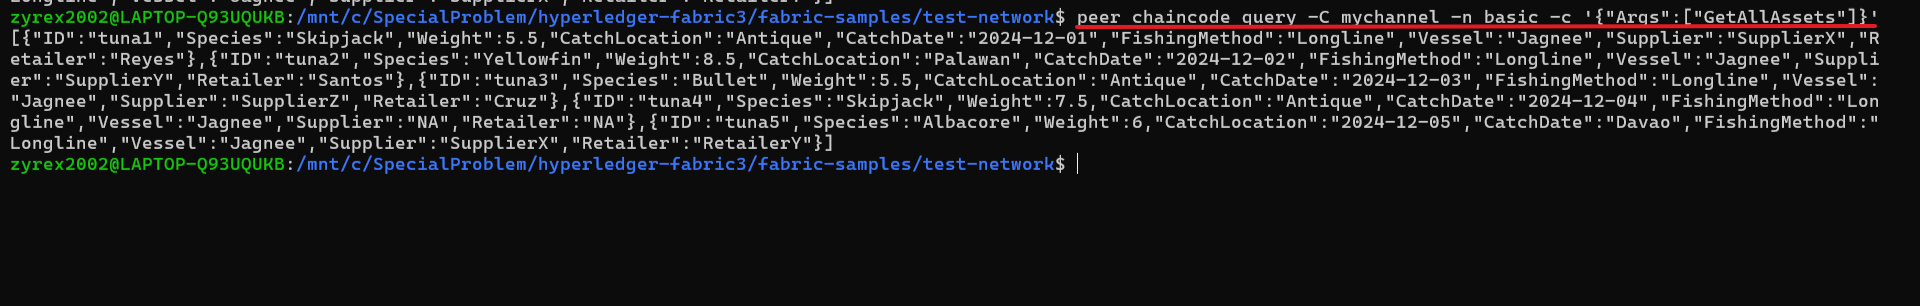
\includegraphics[width=0.8\textwidth]{invoke step 2.png}
		\caption{Query Smart Contract: Check assets}
		\label{fig: second step}
	\end{figure}
	
	\begin{itemize}
	\item \textbf{Adding new tuna assets:}\\
	Here, a new tuna asset is created and registered on the blockchain. This involves invoking the smart contract to add a new entry, which includes details such as the type of tuna, quantity, and any other relevant information. This step ensures that newly caught or acquired tuna can be tracked throughout the supply chain.
	
	\begin{figure}[H]
		\centering
		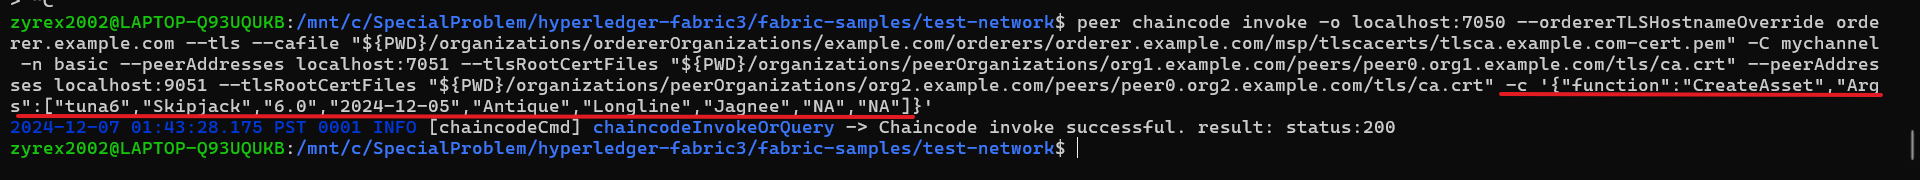
\includegraphics[width=0.8\textwidth]{invoke step 3.png}
		\caption{Invoke Smart Contract: Create/Add new tuna asset}
		\label{fig: third step}
	\end{figure}
	
	\item \textbf{Check all assets after adding a new tuna asset:}\\
	After adding a new tuna asset, the smart contract is queried again to verify that the asset has been successfully added. This step confirms that the new asset is part of the current inventory and that no discrepancies exist in the recorded data.
	
	\begin{figure}[H]
		\centering
		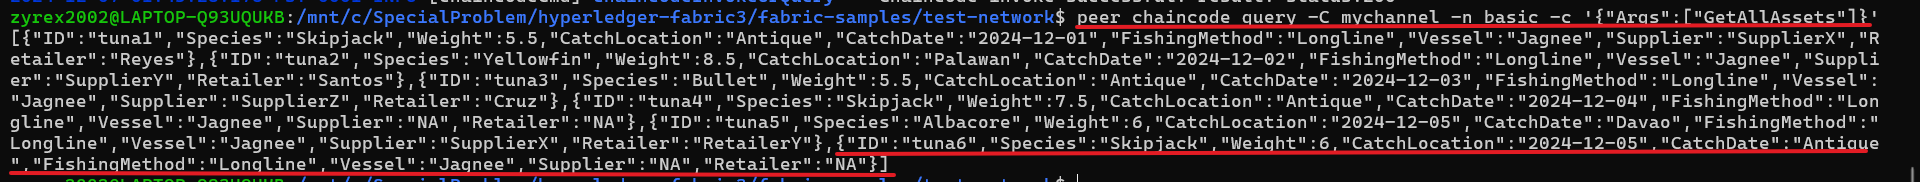
\includegraphics[width=0.8\textwidth]{invoke step 4.png}
		\caption{Query Smart Contract: Check assets with new tuna asset}
		\label{fig: fourth step}
	\end{figure}
	
	\item \textbf{Transfer tuna asset to Supplier:}\\
	This step involves transferring ownership of a tuna asset from the current holder (e.g., a fisherman or a trader) to a supplier. The smart contract is invoked to facilitate the transfer, ensuring that the transaction is securely recorded on the blockchain and that the asset’s new owner is updated accordingly.
	
	\begin{figure}[H]
		\centering
		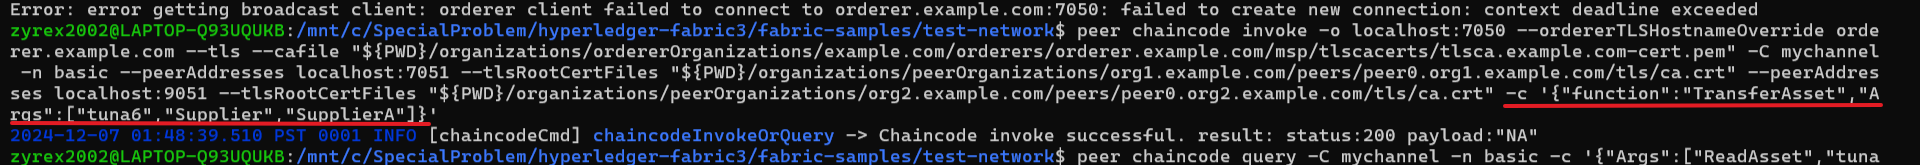
\includegraphics[width=0.8\textwidth]{invoke step 5.png}
		\caption{Invoke Smart Contract: Transfer asset to a supplier}
		\label{fig: fifth step}
	\end{figure}
	
	\item \textbf{Check the updated tuna asset:}\\
	After the transfer, the smart contract is queried once more to check if the asset details have been updated correctly. This step verifies that the asset’s new owner is now the supplier and that all relevant information is correctly updated on the blockchain.
	
	\begin{figure}[H]
		\centering
		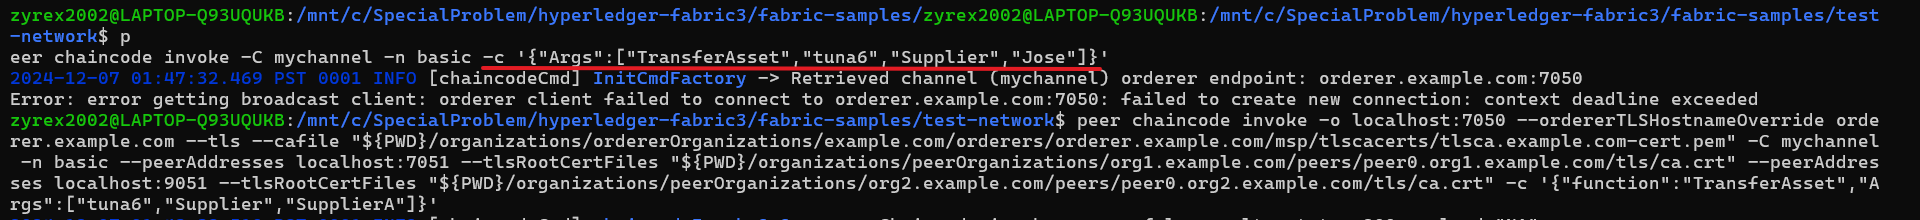
\includegraphics[width=0.8\textwidth]{invoke step 6.png}
		\caption{Query Smart Contract: Check asset after transfer}
		\label{fig: sixth step}
	\end{figure}
	
	\item \textbf{Transfer tuna asset to Retailer:}\\
	Similar to the supplier transfer, this step involves transferring the tuna asset from the supplier to a retailer. The smart contract facilitates this transfer, ensuring that ownership is correctly updated and that the retailer has control over the tuna asset. This step is crucial for the supply chain as it moves the tuna from bulk supply to retail.
	
	\begin{figure}[H]
		\centering
		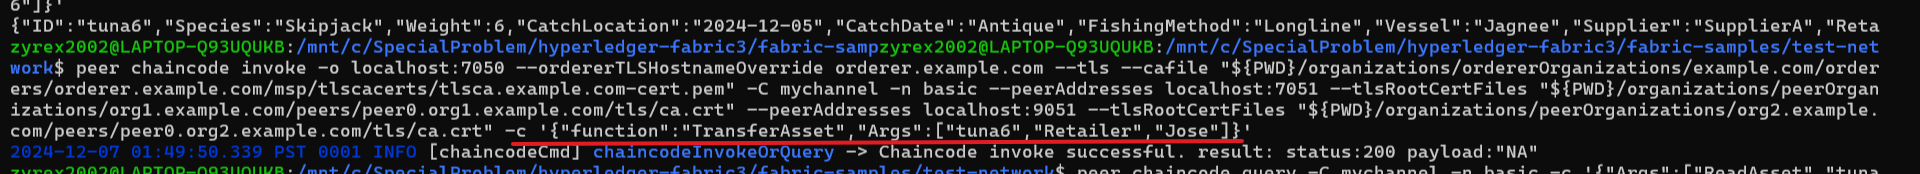
\includegraphics[width=0.8\textwidth]{invoke step 7.png}
		\caption{Invoke Smart Contract: Transfer asset to a retailer}
		\label{fig: seventh step}
	\end{figure}
	
	\item \textbf{Check the updated tuna asset:}\\
	After the transfer to the retailer, another query is made to verify the updated asset details. This step ensures that the transaction was successful and that the retailer now has ownership of the tuna asset. It confirms that the asset has moved through the supply chain correctly.
	
	\begin{figure}[H]
		\centering
		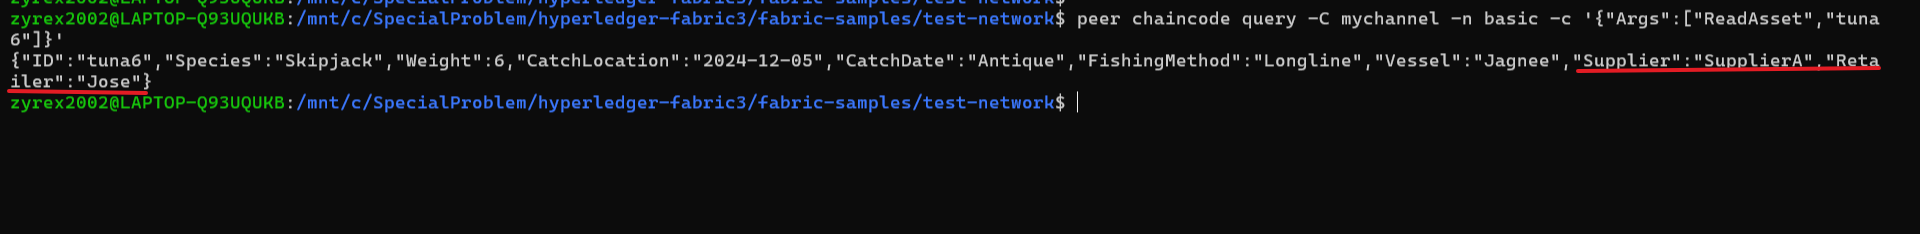
\includegraphics[width=0.8\textwidth]{invoke step 8.png}
		\caption{Query Smart Contract: Check asset after transfer}
		\label{fig: eight step}
	\end{figure}
	
	\item \textbf{Query Smart Contract and check updated assets:}\\
	The final step involves querying the smart contract to get a complete overview of all the assets in the supply chain. This includes all tuna assets from fishing to retail, allowing stakeholders to monitor and manage inventory effectively. It provides traceability in the supply chain, helping to maintain freshness and authenticity of the tuna as it moves through the market.
	
	\begin{figure}[H]
		\centering
		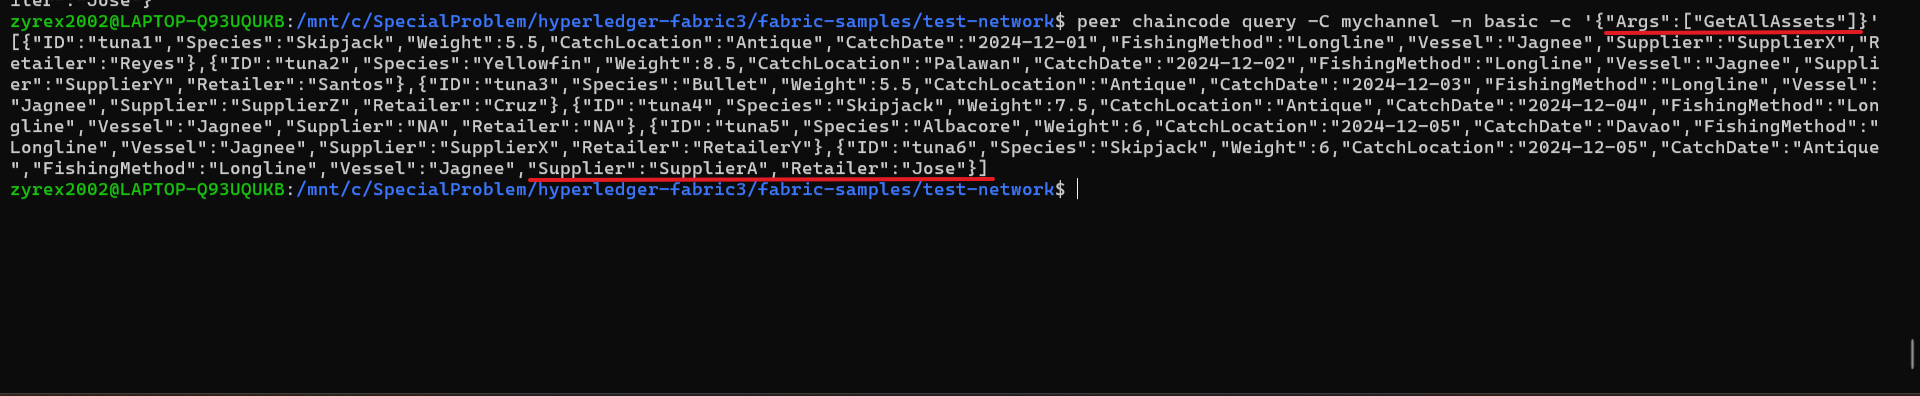
\includegraphics[width=0.8\textwidth]{invoke step 9.png}
		\caption{Query Smart Contract: Check updated assets}
		\label{fig: ninth step}
	\end{figure}
	
		
	\end{itemize}
\section{Backend Security Analysis (Hyperledger Fabric on GCP)}

\subsection{System Architecture and Deployment Overview}
The backend of the system’s tuna assets was developed using a containerized Hyperledger Fabric deployed on Google Cloud Platform (GCP). The network of Hyperledger Fabric consists of a peer node, an ordering node, and Certificate Authorities (CAs). 

\subsection{Blockchain Network Security}
The blockchain network leverages Hyperledger Fabric’s security model to ensure authenticated transactions and controlled access. A Membership Service Provider (MSP) manages identities and issues certificates based on a Public Key Infrastructure (PKI) model, ensuring that only verified participants can interact with the network.

Key security features include:

\subsubsection{Channel Privacy}
Channels act as private communication subnets, isolating transaction data so that only authorized organizations can access and process specific transactions.

\subsubsection{Policies and Access Control}
Policies, including endorsement policies and access control lists (ACLs), govern how transactions are validated, how channel resources are accessed, and how changes to the network are approved. Endorsement policies specifically define which peer nodes must approve a transaction before it is committed to the ledger.

\subsubsection{Secure Communication}
Transport Layer Security (TLS) is enforced across node communications to protect data in transit. Mutual TLS is used for operational endpoints like monitoring services.

\subsubsection{Identity and Role Management}
Every network participant—peer nodes, orderer nodes, client applications (SeaXChange Web Application)—has a cryptographically verifiable identity, with roles defined within the framework to control access and permissions within channels.

\subsubsection{Hardware Security Modules (HSMs)}
Critical cryptographic operations, such as signing transactions under the blockchain assets invocation, can optionally be handled by HSMs to secure private keys outside of the software environment.

These layered mechanisms collectively ensure the confidentiality, integrity, and authenticity of transactions in the blockchain network.

\subsection{Smart Contract Automated Test Result}
To validate the security and functionality of the deployed smart contracts on the Hyperledger Fabric network, an automated testing script (app.js) under asset-transfer-basic directory was executed. The script interacted with the blockchain network through the gateway application, utilizing the defined channel (mychannel) and chaincode (basic). The automated tests performed the following operations:

\subsubsection{InitLedger Transaction}
The ledger was initialized by creating a predefined set of tuna asset entries. The transaction was successfully committed, confirming the proper initialization of asset data.
(See Figure \ref{fig:initledger} for initialization confirmation.)

\begin{figure}[H]
	\centering
	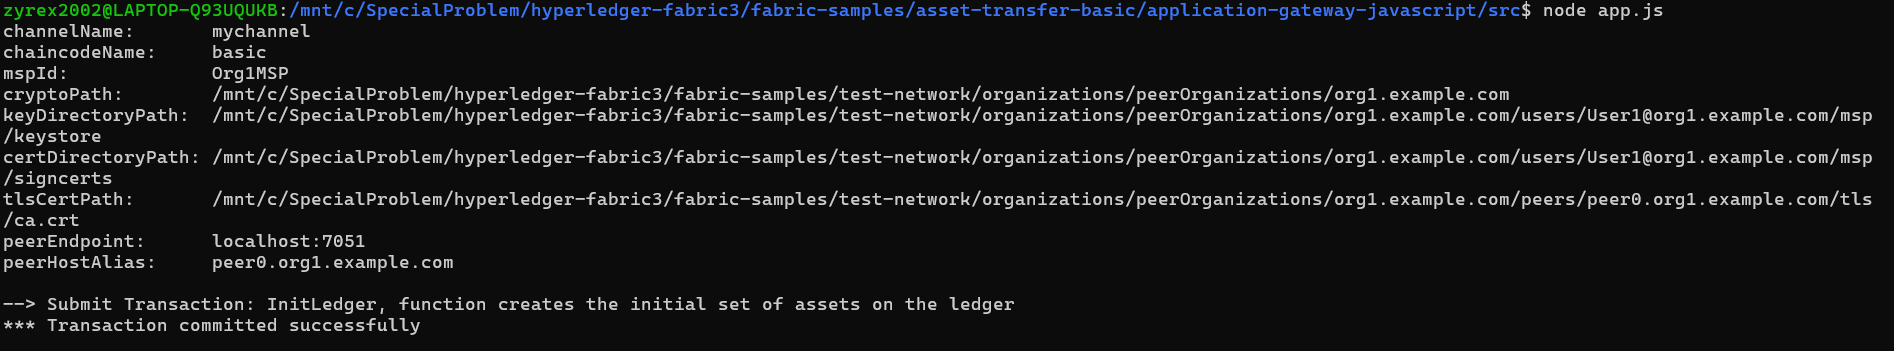
\includegraphics[width=0.8\textwidth]{chaincode_security1.png} % Adjust the path and size as needed
	\caption{Initialization Confirmation of the Ledger}
	\label{fig:initledger}
\end{figure}


\subsubsection{GetAllAssets Query}
A query operation retrieved all existing assets recorded on the ledger. The results displayed multiple tuna asset entries with details such as species, weight, catch location, catch date, fishing method, fisher, supplier, retailers, selling locations, and consumers.
(See Figure \ref{fig:getallledger} for the asset retrieval output.)

\begin{figure}[H]
	\centering
	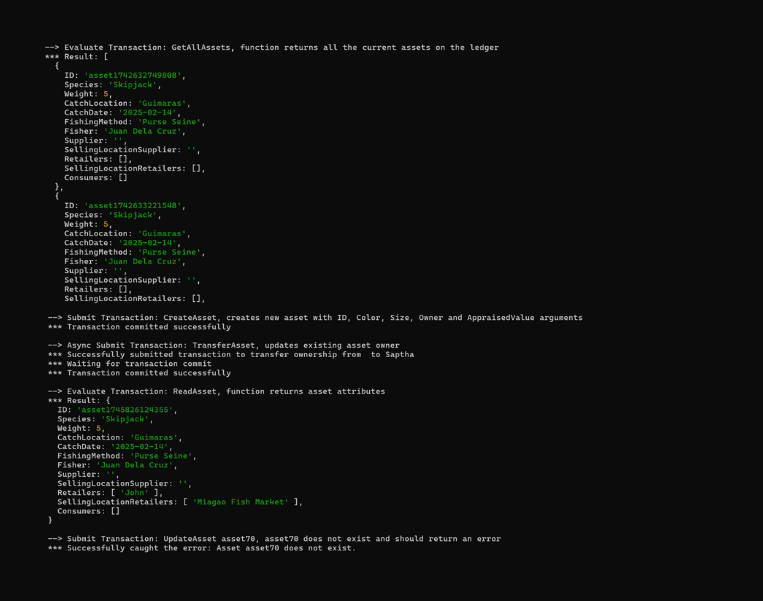
\includegraphics[width=0.8\textwidth]{chaincode_security2.png} % Adjust the path and size as needed
	\caption{Initialization Confirmation of the Ledger}
	\label{fig:getallledger}
\end{figure}

\subsubsection{CreateAsset Transaction}
A new asset was successfully created and appended to the blockchain. The transaction was committed without errors, validating the chaincode’s ability to handle new data insertion.

\subsubsection{TransferAsset Transaction}
Ownership transfer of an existing asset was simulated. The transaction was successfully submitted and committed, demonstrating the correct application of asset updates in the blockchain ledger.

\subsubsection{ReadAsset Query}
The updated asset was retrieved and verified to ensure the correctness of the transfer. The retrieved asset data reflected the changes made through the previous transaction, confirming data consistency.

\subsubsection{UpdateAsset Error Handling}
An attempt to update a non-existent asset (asset70) was performed to test the smart contract’s error-handling mechanism. The application correctly caught and reported the error, verifying that improper transactions are adequately handled and rejected.

\subsubsection{Summary of Results}
All positive transactions (initialization, creation, transfer, and reading) were successfully executed and committed. The smart contract exhibited robust error handling during invalid operations. Endorsement policies and Membership Service Provider (MSP) enforcement ensured transaction authenticity and integrity during the process. These tests confirm the functional reliability and transaction security of the smart contracts used within the tuna supply chain blockchain network.

\subsection{GCP Infrastructure Security}
The Hyperledger Fabric network deployment on Google Cloud Platform (GCP) was secured by leveraging multiple layers of Google's infrastructure security model, following best practices in network, identity, and data protection.

\subsubsection{Firewall Rules and Network Control}
Only essential ports (e.g., 7051 for peer communication and 7050 for the ordering service) were opened to minimize network exposure. GCP’s VPC firewall rules, ingress and egress controls, and options like VPC Service Controls help further isolate services and prevent unauthorized access. Traffic between virtual machines and Google APIs is securely routed through Google’s internal network infrastructure using Private Google Access when available.

\subsubsection{IAM Roles and Access Management}
The principle of least privilege was enforced by assigning minimal permissions to users and services through GCP Identity and Access Management (IAM). Access decisions involve authentication, authorization checks, and enforcement of policies through centralized services, helping reduce the risk of unauthorized actions or privilege escalation.

\subsubsection{Encryption}
GCP ensures that data is encrypted both at rest and in transit by default. Storage systems use multiple layers of encryption, with cryptographic keys managed by Google. For additional control, Cloud Key Management Service (KMS) enables customers to manage their own encryption keys. Data in transit between services is protected using Application Layer Transport Security (ALTS), and all external communication with Google services is encrypted via TLS.

\subsubsection{Access Control}
Access to virtual machines and services was restricted using secure access methods. Identity-Aware Proxy (IAP) or VPN connections were employed to safeguard SSH and administrative access. GCP’s zero-trust model emphasizes verifying identity and device security rather than relying solely on network location, aligning with best practices for modern infrastructure protection.

\subsubsection{Infrastructure and Operational Security}
GCP's underlying infrastructure benefits from Google's proprietary hardware designs, including the Titan security chip, secure boot mechanisms, and service identity enforcement. Google's physical data centers use multi-layered defenses such as biometrics and intrusion detection systems. Operational security practices, including binary authorization and extensive monitoring, reduce insider risks and enforce software integrity throughout the lifecycle.

\noindent By deploying the blockchain network on GCP, the project leveraged a highly secure environment, benefiting from Google’s layered security architecture across networking, identity management, encryption, access control, and operational practices.

\subsection{Threat Model and Mitigations}
Potential threats to the system were identified and mitigation strategies were applied, as summarized in Table~\ref{tab:threat}.
\begin{table}[h]
	\centering
	\begin{tabular}{|c|c|}
		\hline
		\textbf{Threat} & \textbf{Mitigation} \\
		\hline
		Unauthorized access to network & Use of MSP and Certificate Authorities \\
		\hline
		Tampering with transactions & Endorsement policies and consensus mechanisms \\
		\hline
		Denial of Service (DoS) attacks & GCP Firewall and rate limiting rules \\
		\hline
		Data leakage & Private channels and access controls \\
		\hline
	\end{tabular}
	\caption{Potential Threat and Mitigation}
	\label{tab:threat}
\end{table}


\section{Mockups}
\begin{figure}[H]
	\centering
	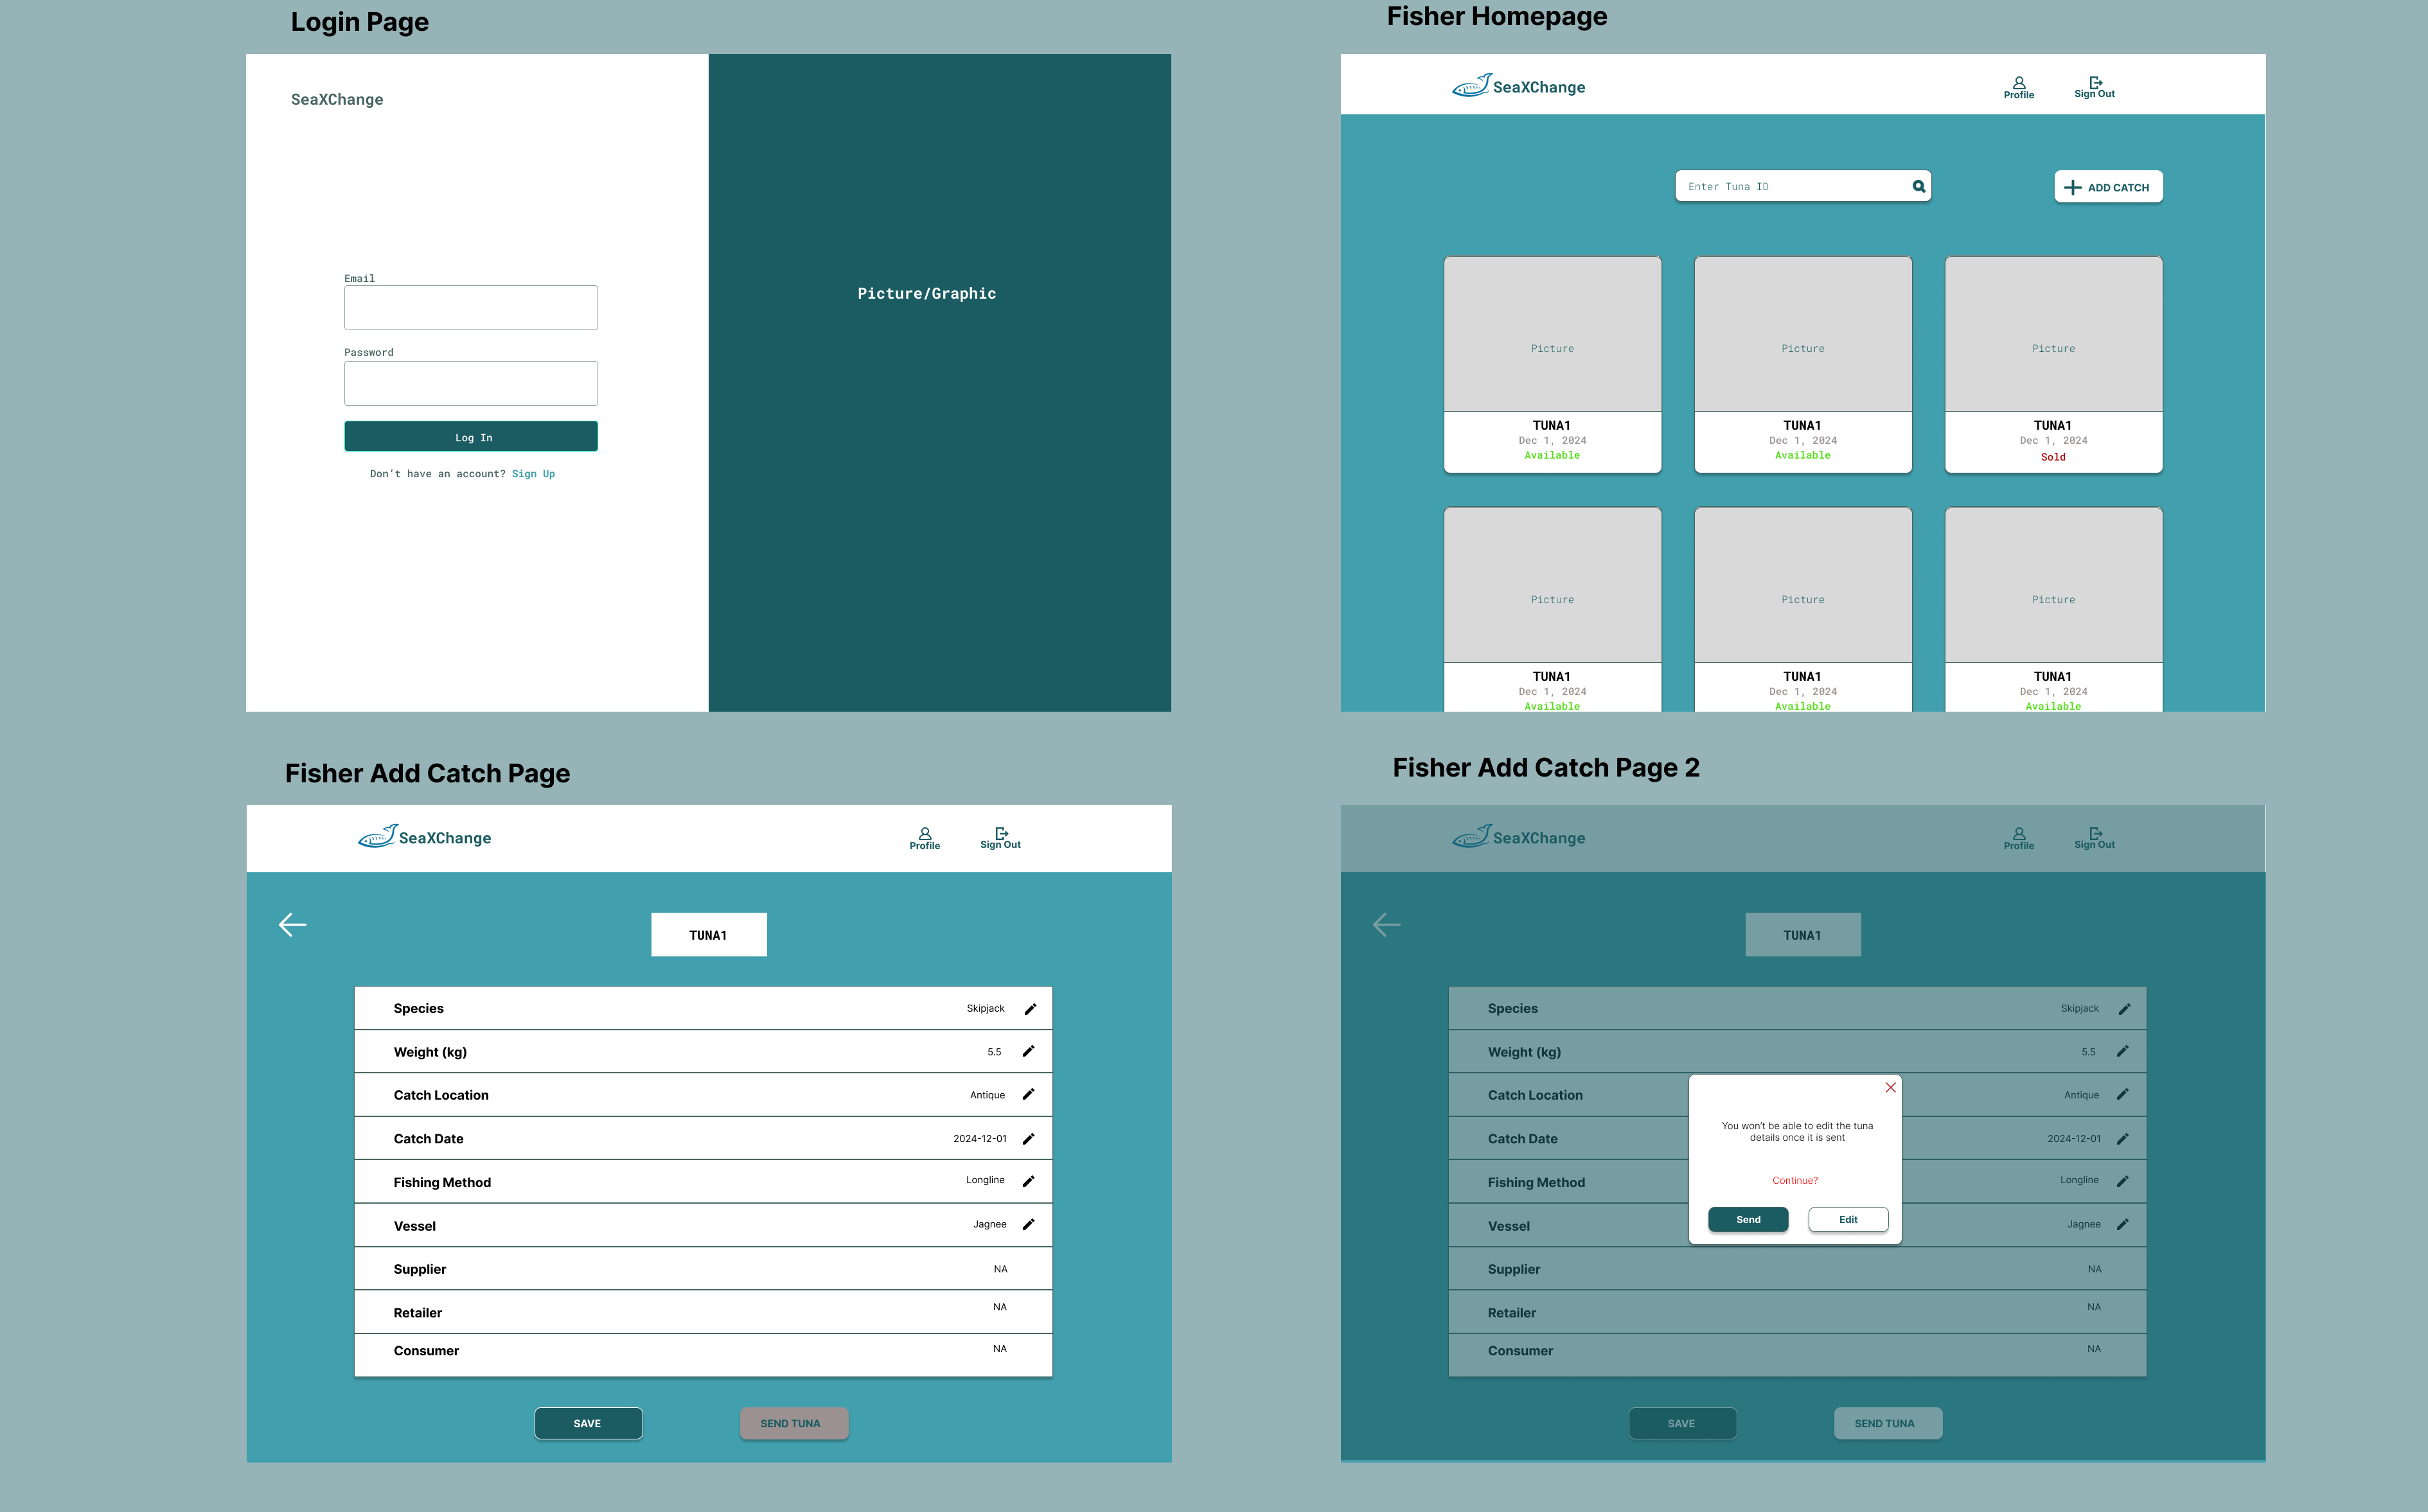
\includegraphics[width=0.9\textwidth]{mockup1.png}
	
	\vspace{20pt} % Adjust space 
	
	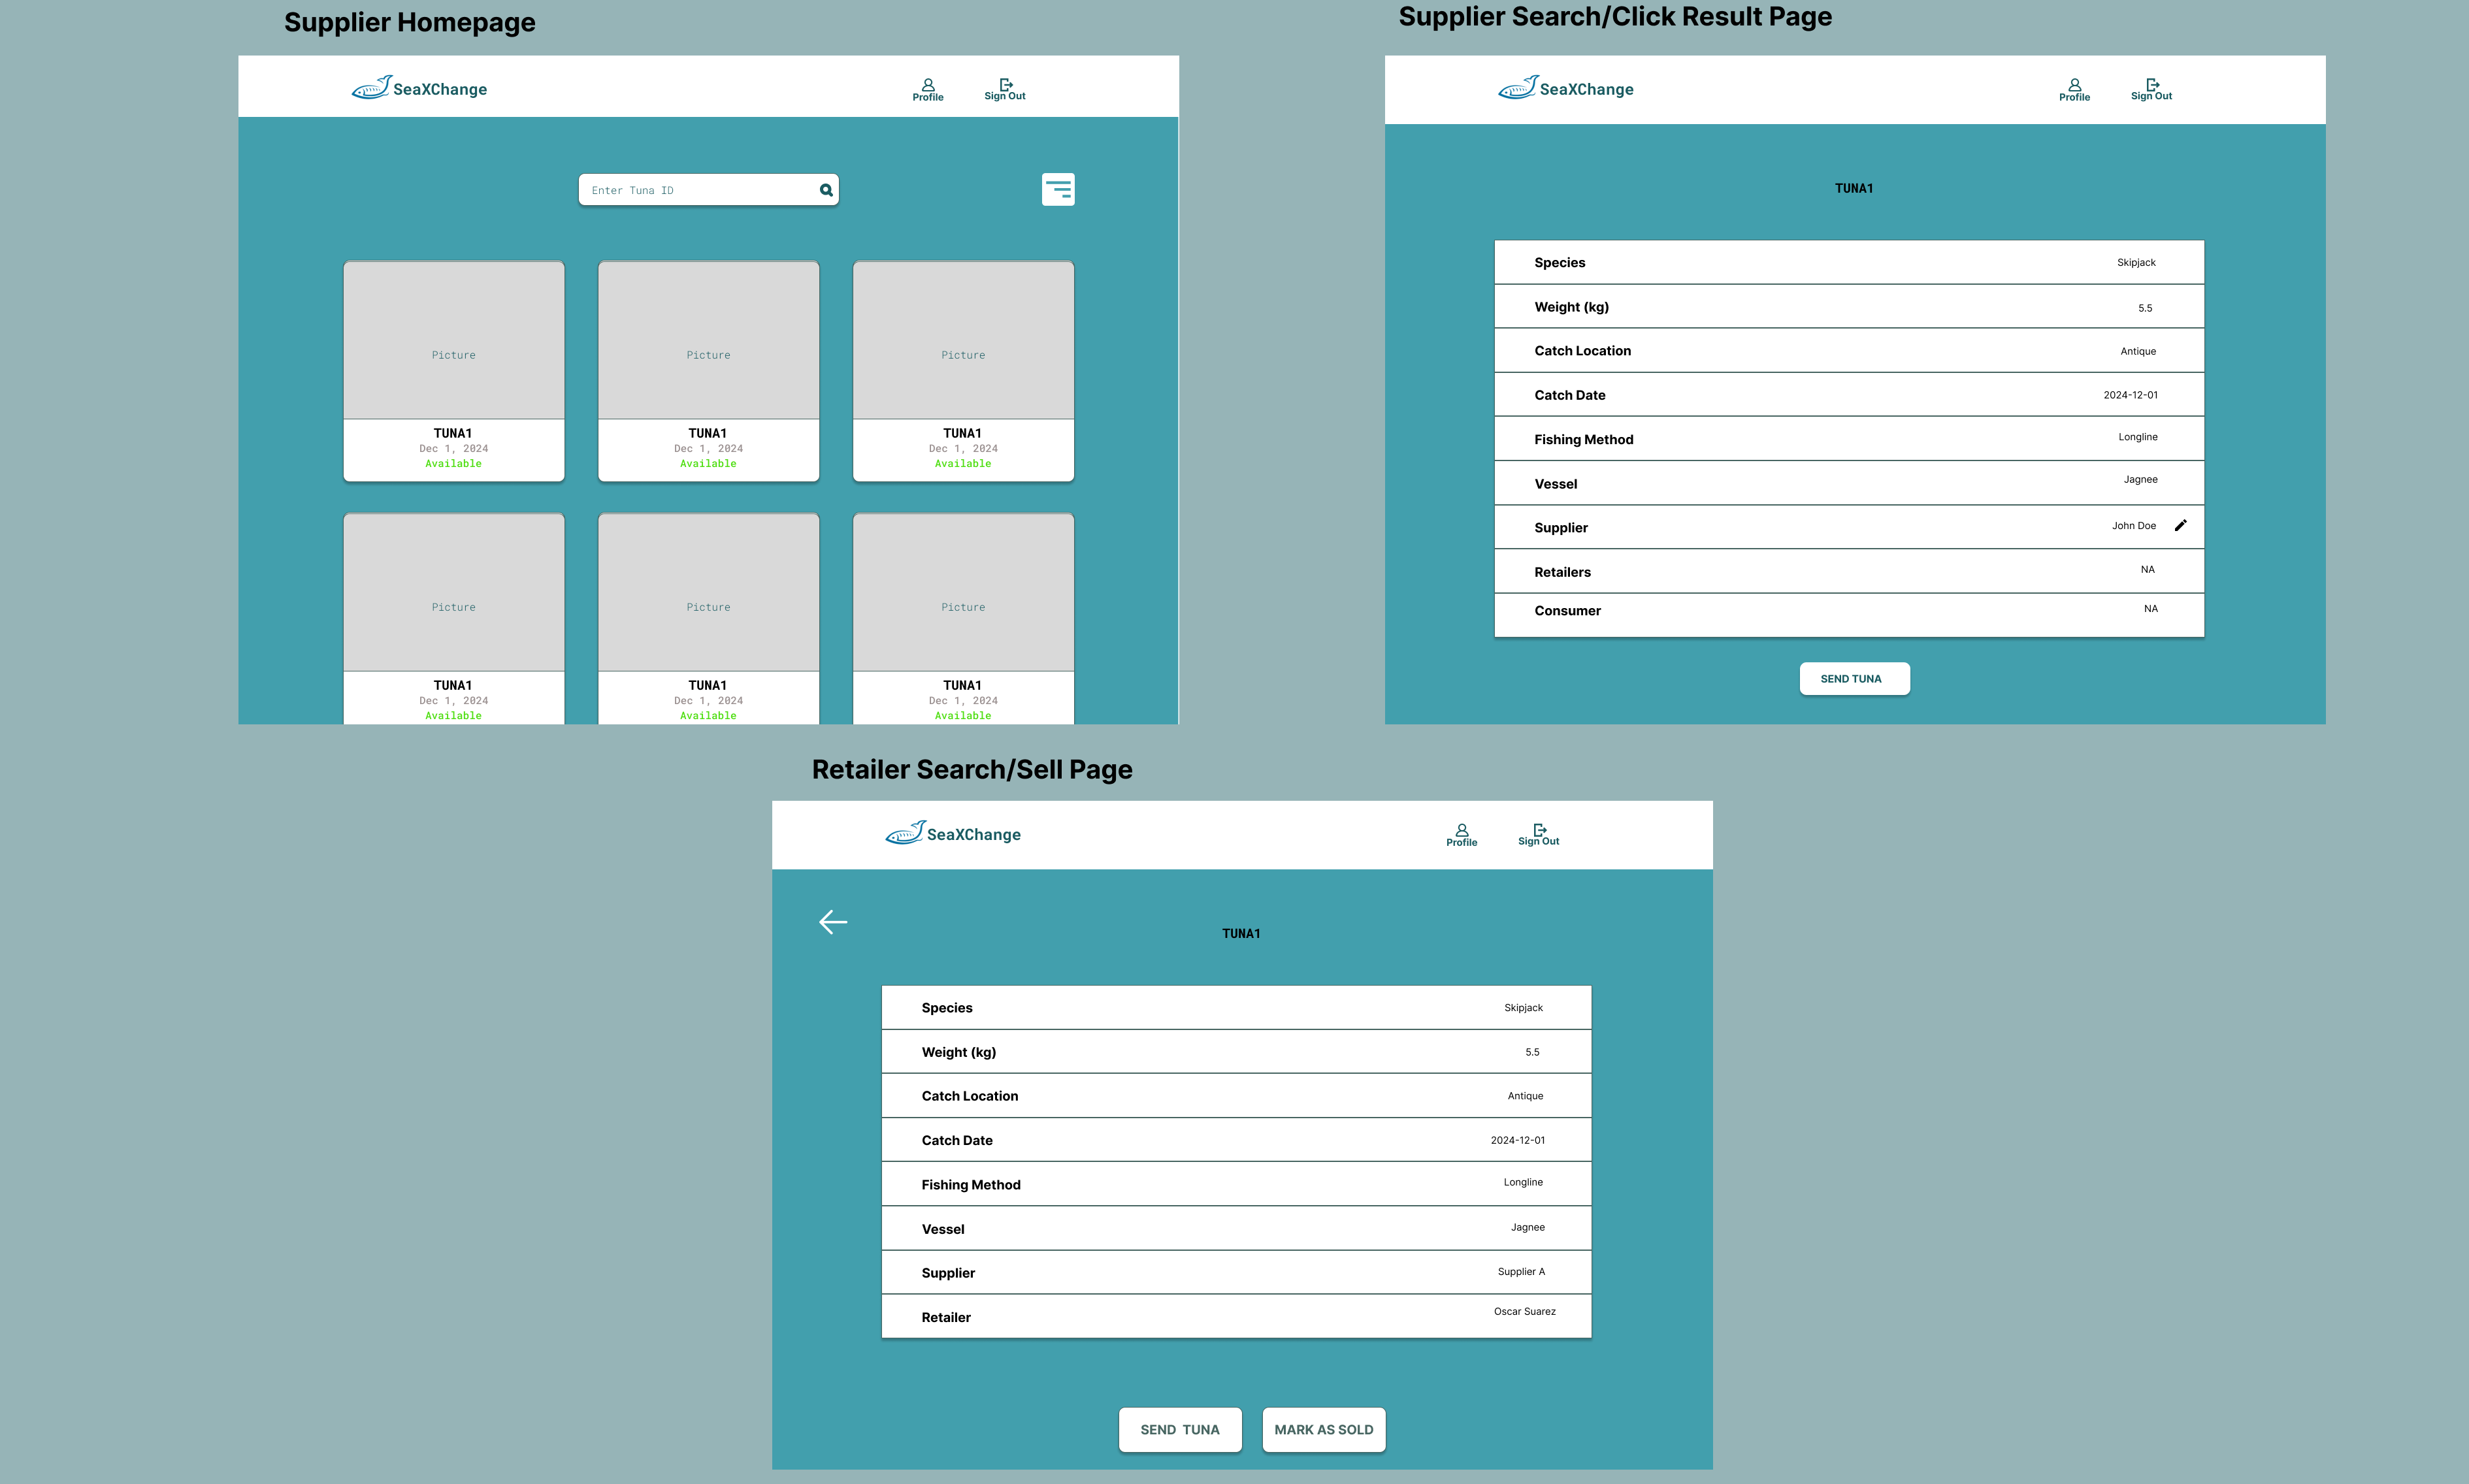
\includegraphics[width=0.9\textwidth]{mockup2.png}
\end{figure}

\clearpage % Forces the next content to a new page


\begin{figure}[H]
	\centering
	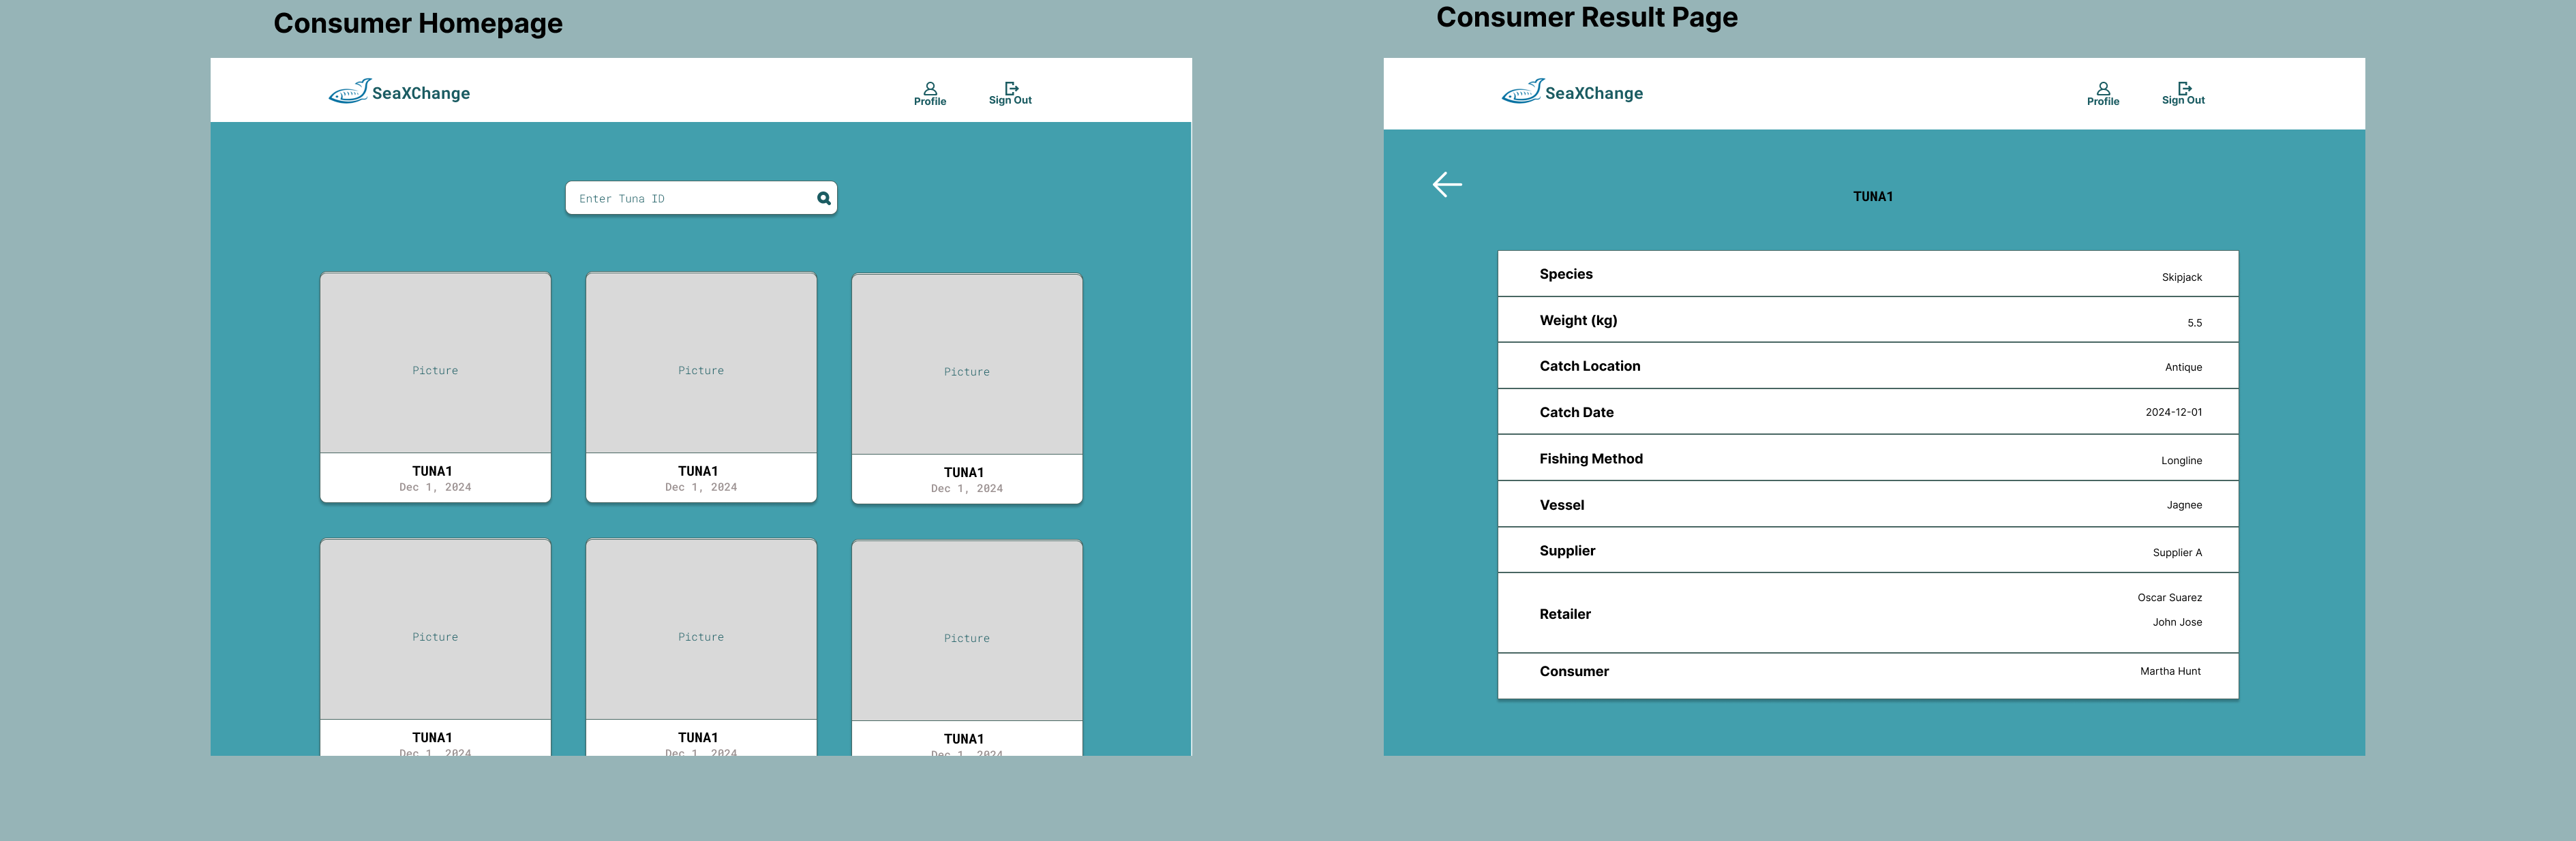
\includegraphics[width=0.9\textwidth]{mockup3.png}
	\caption{SeaXChange Mockups}
	\label{fig:eight_step}
\end{figure}


\section{Operational Flow of the Web Application}
This will discuss the flow in using the SeaXChange Web Application.

\subsection{Landing Page}
Users are be greeted with the landing page, where it shows a ocean visuals and a tagline “Discover the Journey your tuna made from the ocean to your dinner plate”. Users are given the option to Login, where they are redirected to the login page or Get Started, where they are redirected to the sign up page. 

	\begin{figure}[H]
		\centering
		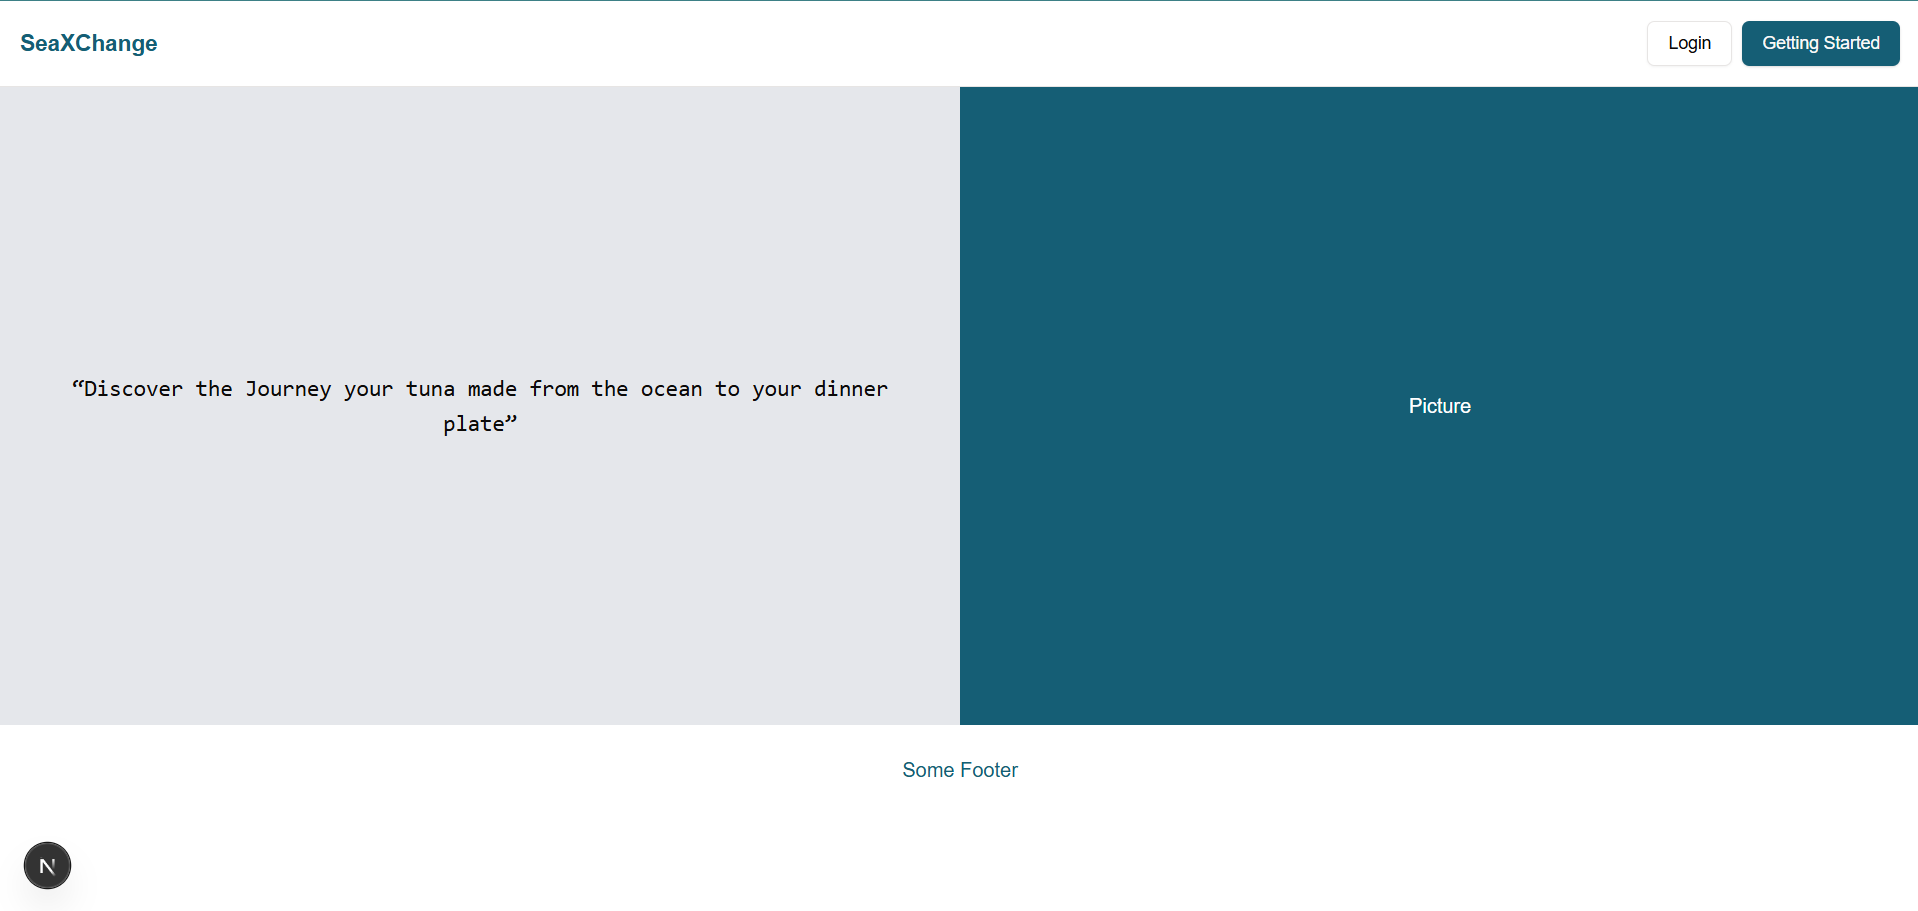
\includegraphics[width=0.8\textwidth]{LandingPage.png}
		\caption{Landing Page}
		\label{fig:landing_page}
	\end{figure}
	
	\begin{figure}[H]
		\centering
		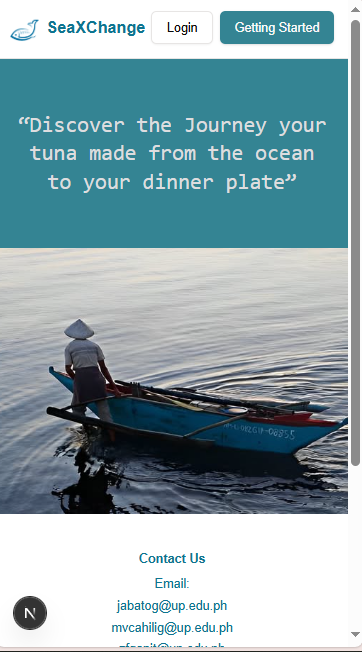
\includegraphics[width=0.8\textwidth]{MobileLandingPage.png}
		\caption{Mobile View: Landing Page}
		\label{fig:mobile_landing_page}
	\end{figure}	

\subsection{Sign Up Page}
First time users will be required to create an account. They are to provide their name, email and password. For their user type, there are four roles to choose from: Fisher, Supplier, Retailer and Consumer. 

	\begin{figure}[H]
		\centering
		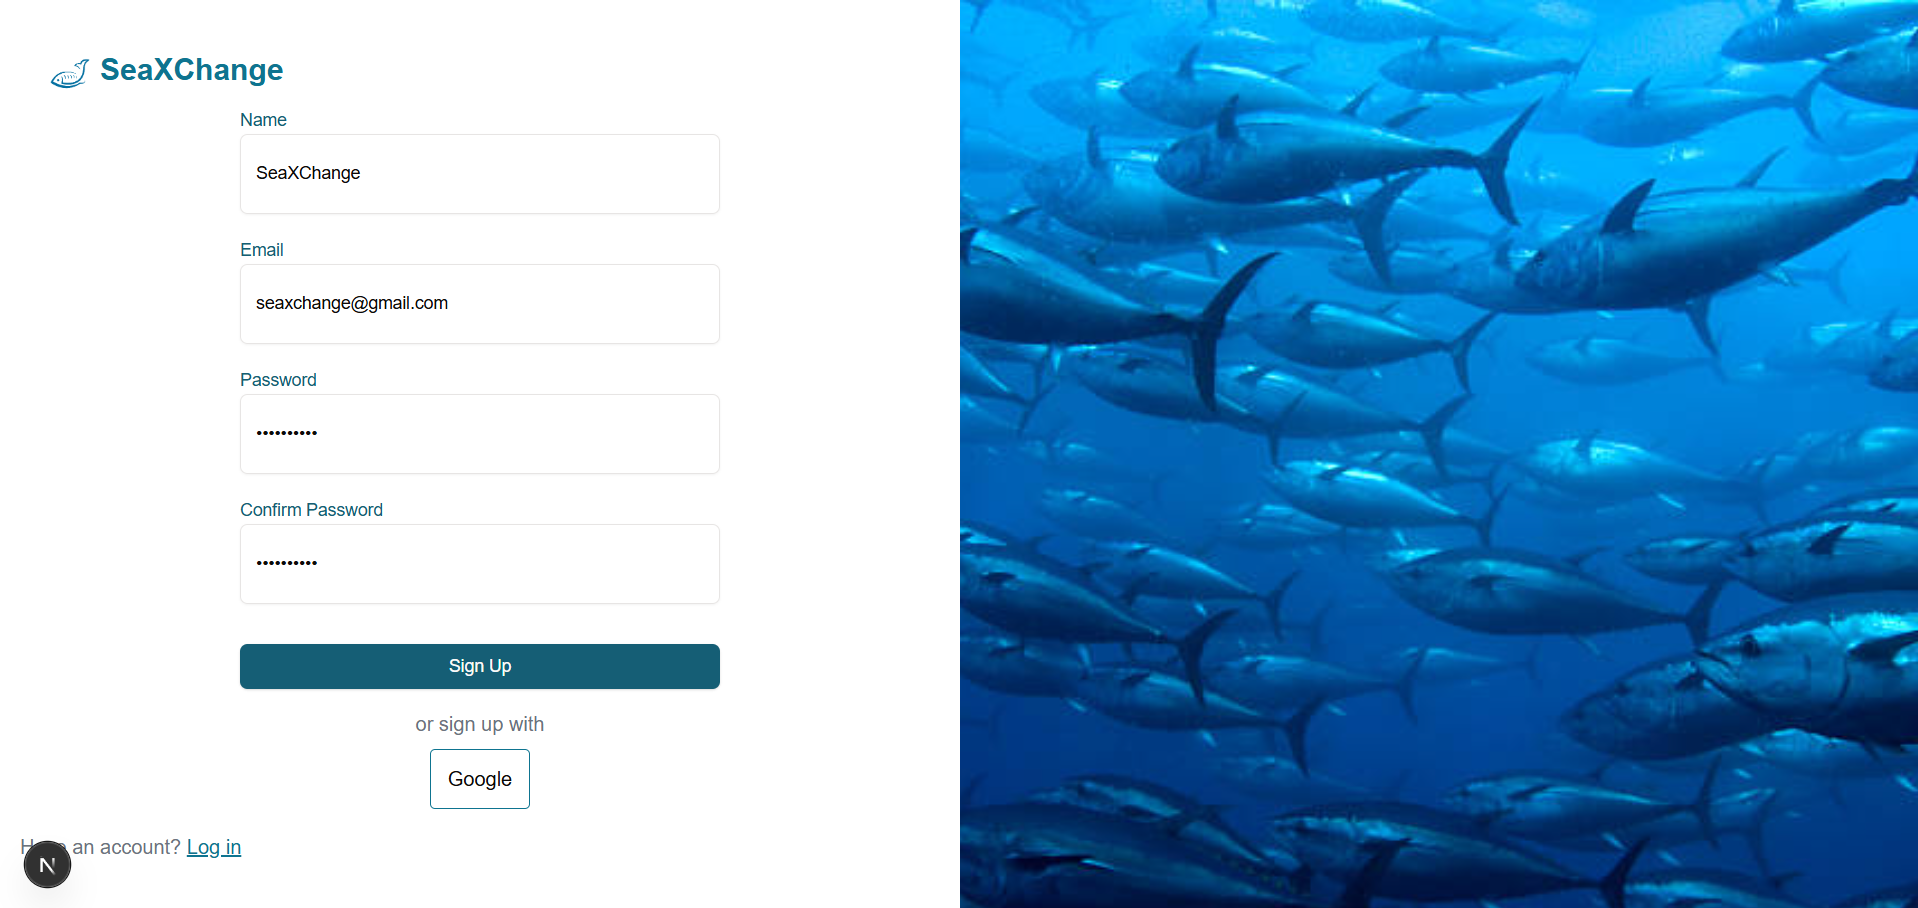
\includegraphics[width=0.8\textwidth]{SignupPage.png}
		\caption{SignUp Page}
		\label{fig:signup_page}
	\end{figure}

\subsection{Login Page}
Returning user are required to login with their email and password.

	\begin{figure}[H]
		\centering
		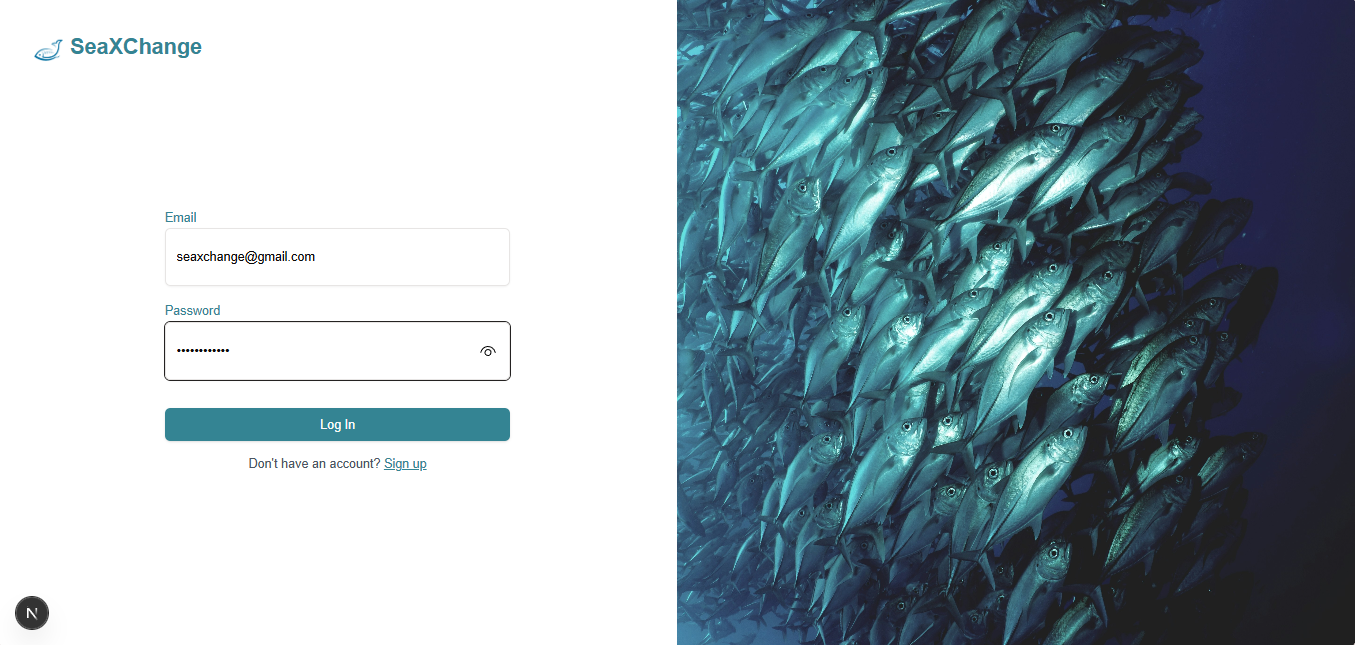
\includegraphics[width=0.8\textwidth]{LoginPage.png}
		\caption{LogIn Page}
		\label{fig:login_page}
	\end{figure}

\subsection{Homepage}
Each user type has their own respective homepages and features.
	\begin{itemize}
		\item \textbf{Fisher}
		Fishers can add a fish catch using the "Add catch" button, where they are to input the species of the fish, weight in kg, catch location, catch date, fishing method used and vessel name. The remaining text fields like the Supplier name, Retailer name and Consumer name are left null and cannot be edited because they will be filled out by the other users receiving the tuna asset. Users can send a tuna asset to the Supplier. Users can also browse existing tuna assets. 
		
			\begin{figure}[H]
				\centering
				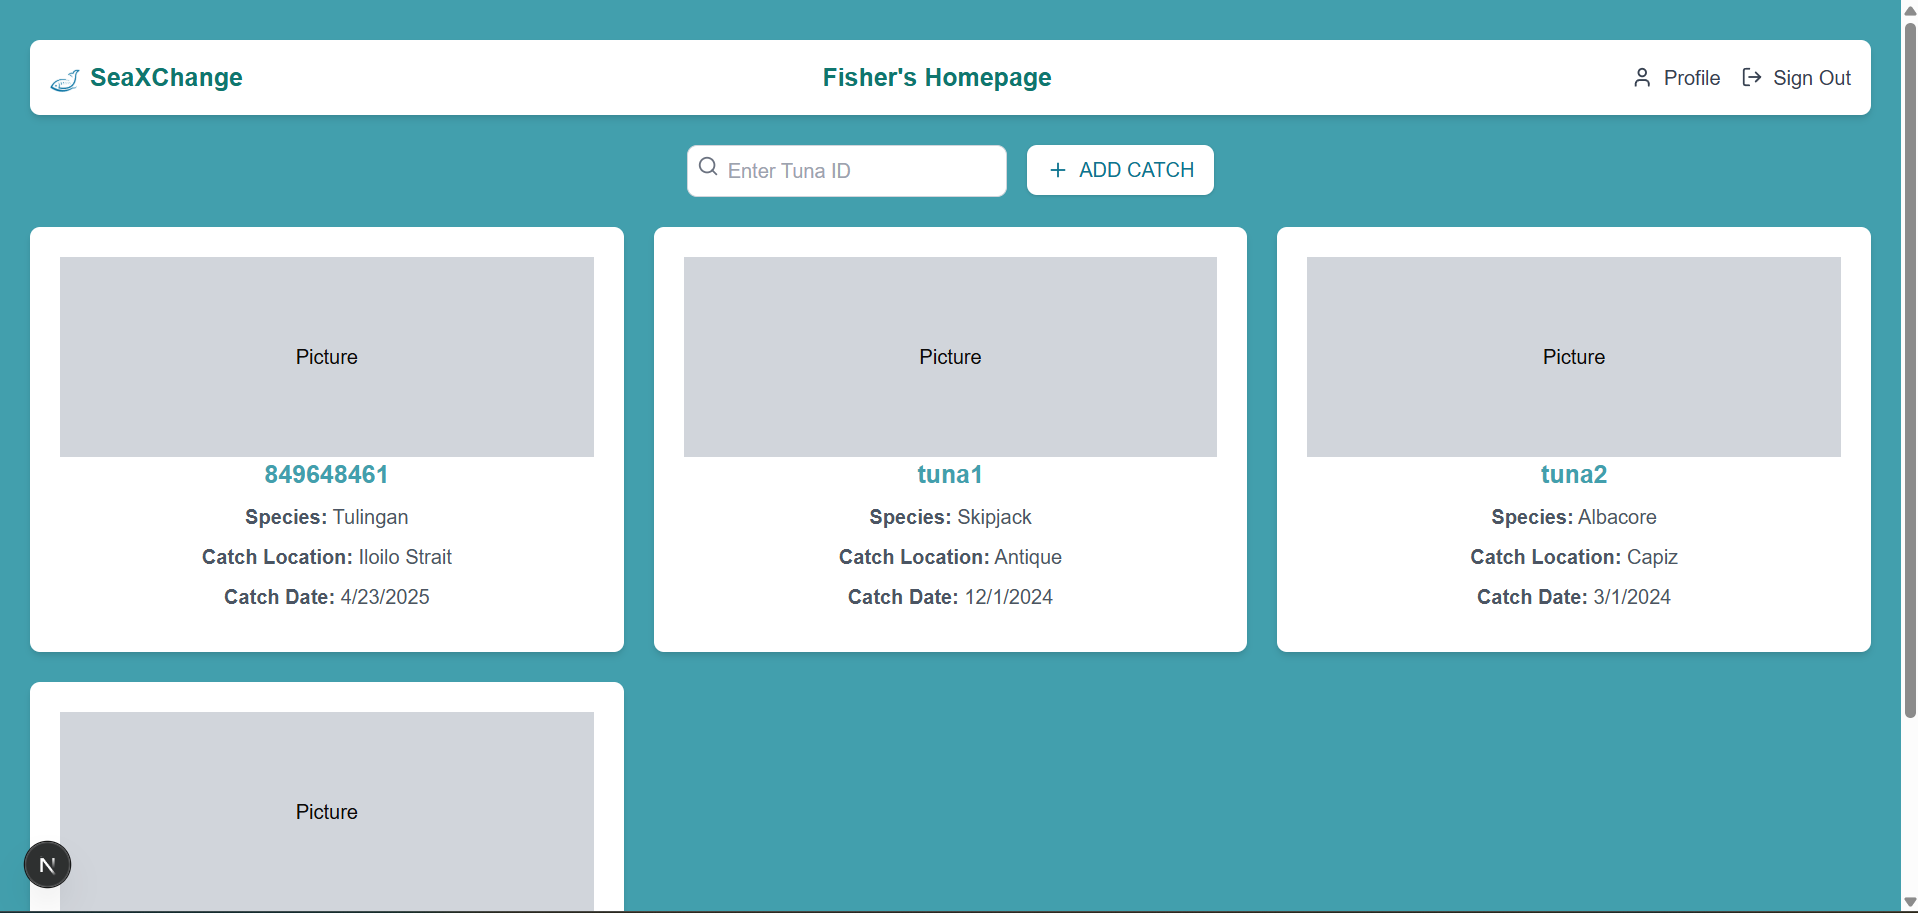
\includegraphics[width=0.8\textwidth]{FisherHomepage.png}
				\caption{Fisher Homepage}
				\label{fig:fisherhome_page}
			\end{figure}
			
		\item \textbf{Supplier}
		Suppliers can browse existing tuna assets. Upon clicking a tuna asset, the user can only edit the Supplier text field. They can send the tuna asset to the Retailer.
		
			\begin{figure}[H]
				\centering
				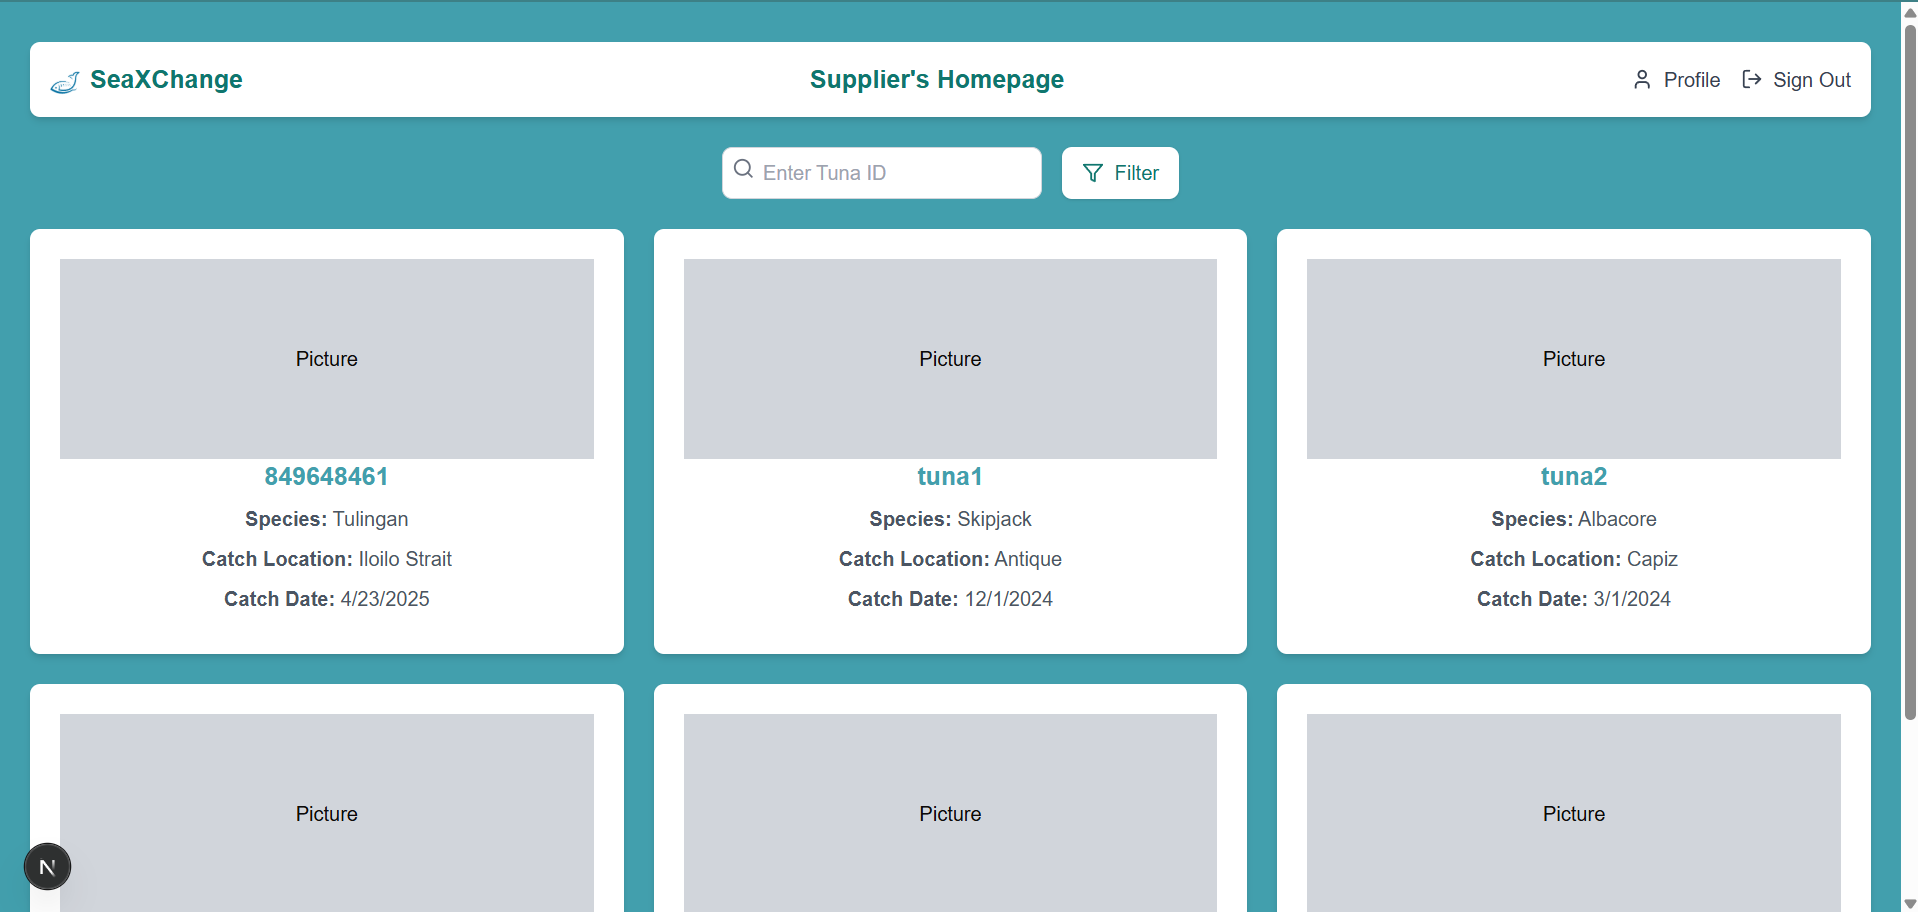
\includegraphics[width=0.8\textwidth]{SupplierHomepage.png}
				\caption{Supplier Homepage}
				\label{fig:supplierhome_page}
			\end{figure}
			
		\item \textbf{Retailer}
		Retailers can browse existing tuna assets and can send it to the Consumer.
		
		\begin{figure}[H]
			\centering
			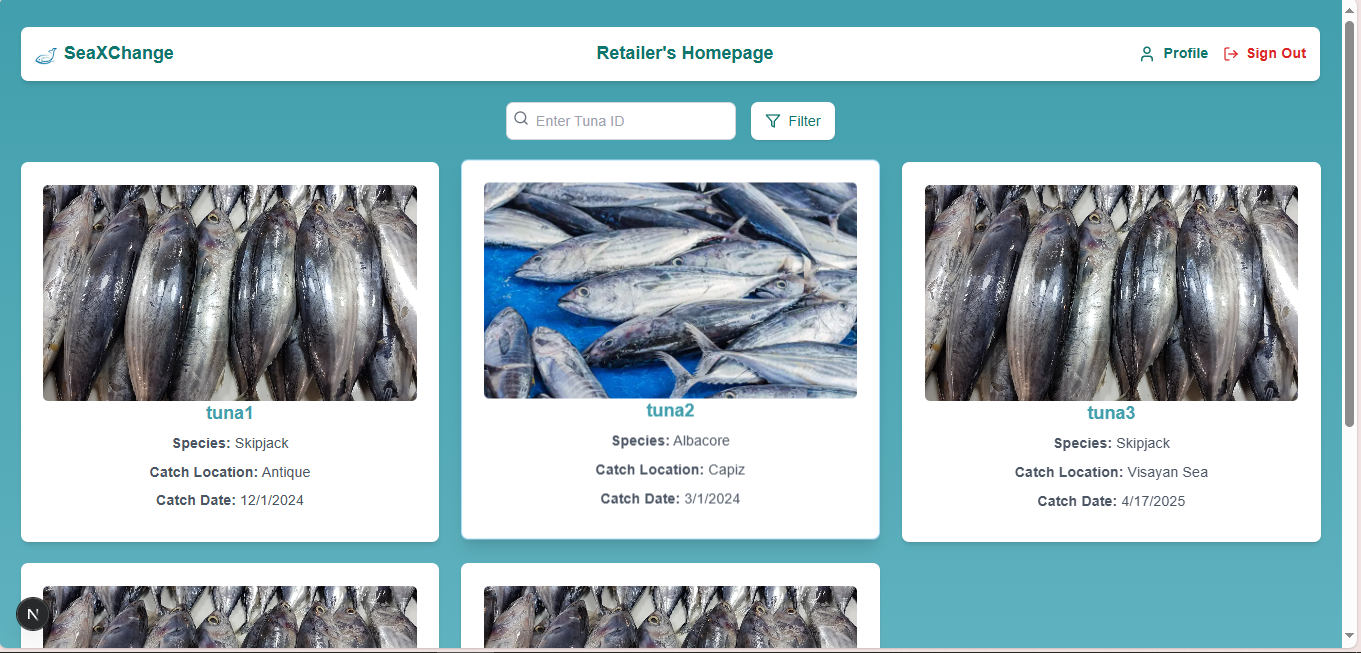
\includegraphics[width=0.8\textwidth]{RetailerHomepage.png}
			\caption{Retailer Homepage}
			\label{fig:retailerhome_page}
		\end{figure}
		
		\item \textbf{Consumer}
		Consumers can only view the tuna asset and cannot edit anything else
		
		\begin{figure}[H]
			\centering
			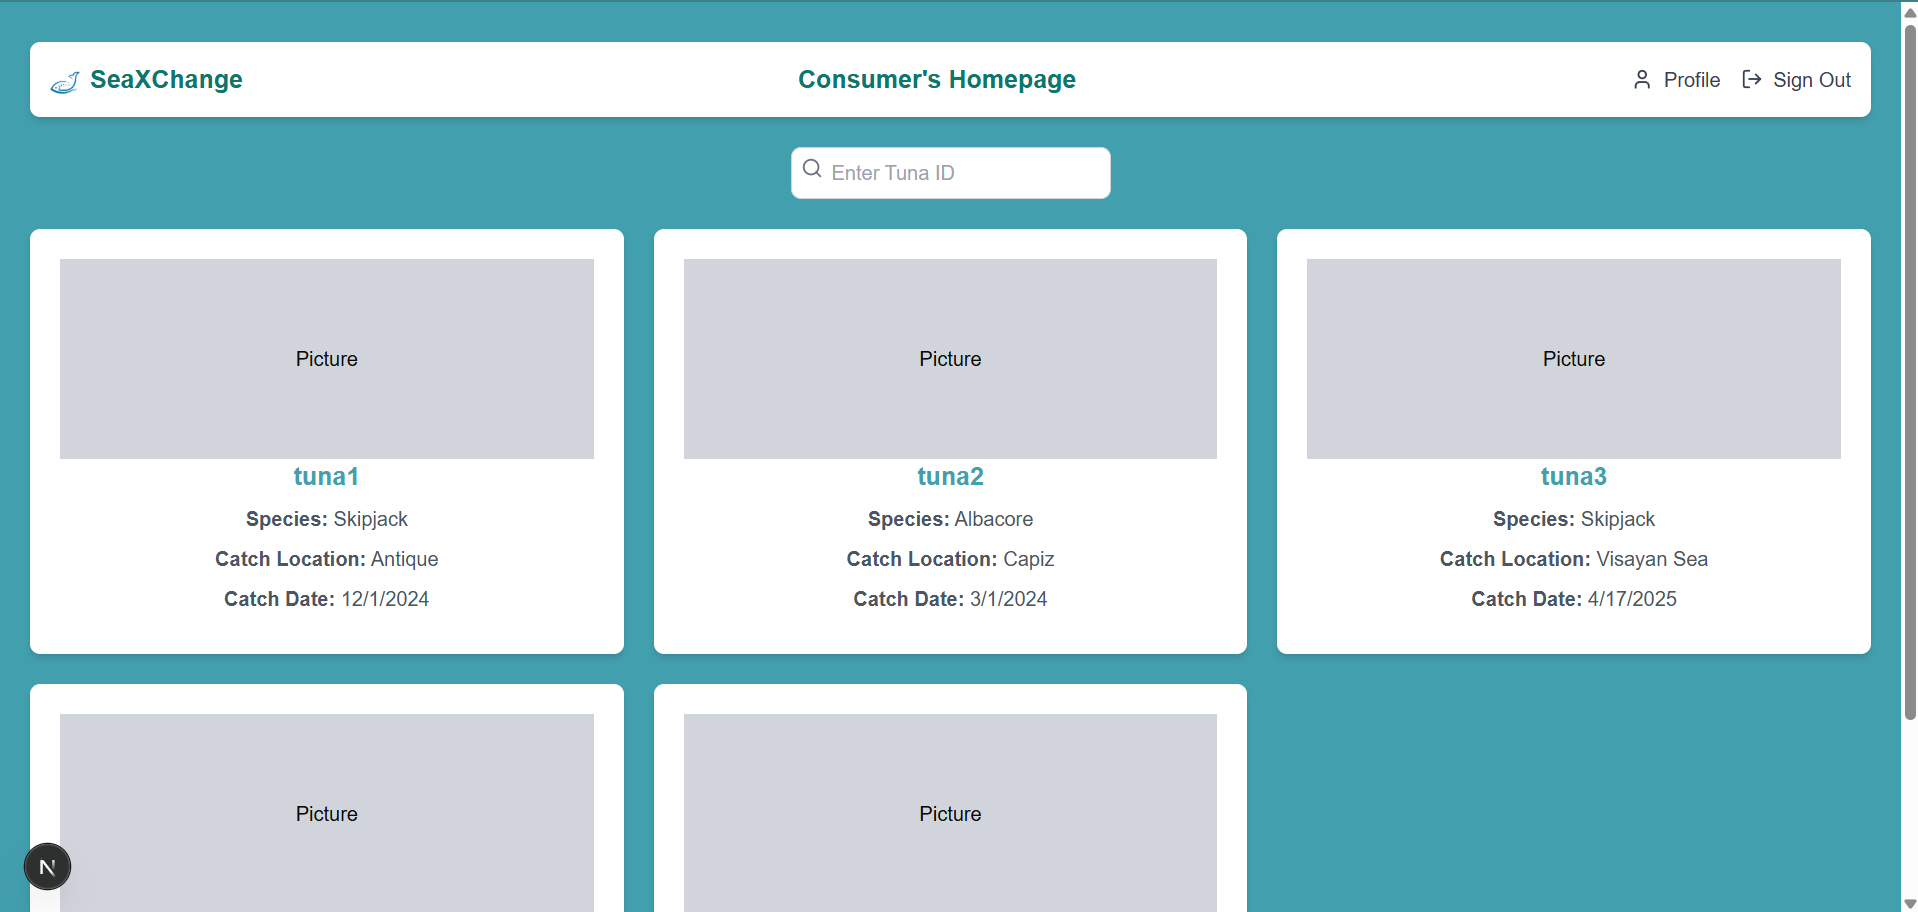
\includegraphics[width=0.8\textwidth]{ConsumerHomepage.png}
			\caption{Consumer Homepage}
			\label{fig:consumerhome_page}
		\end{figure}
		
	\end{itemize}
	
\subsection{Profile}
The user's profile information is shown on the homepage through a pop-up. It shows the user's name and role.

	\begin{figure}[H]
		\centering
		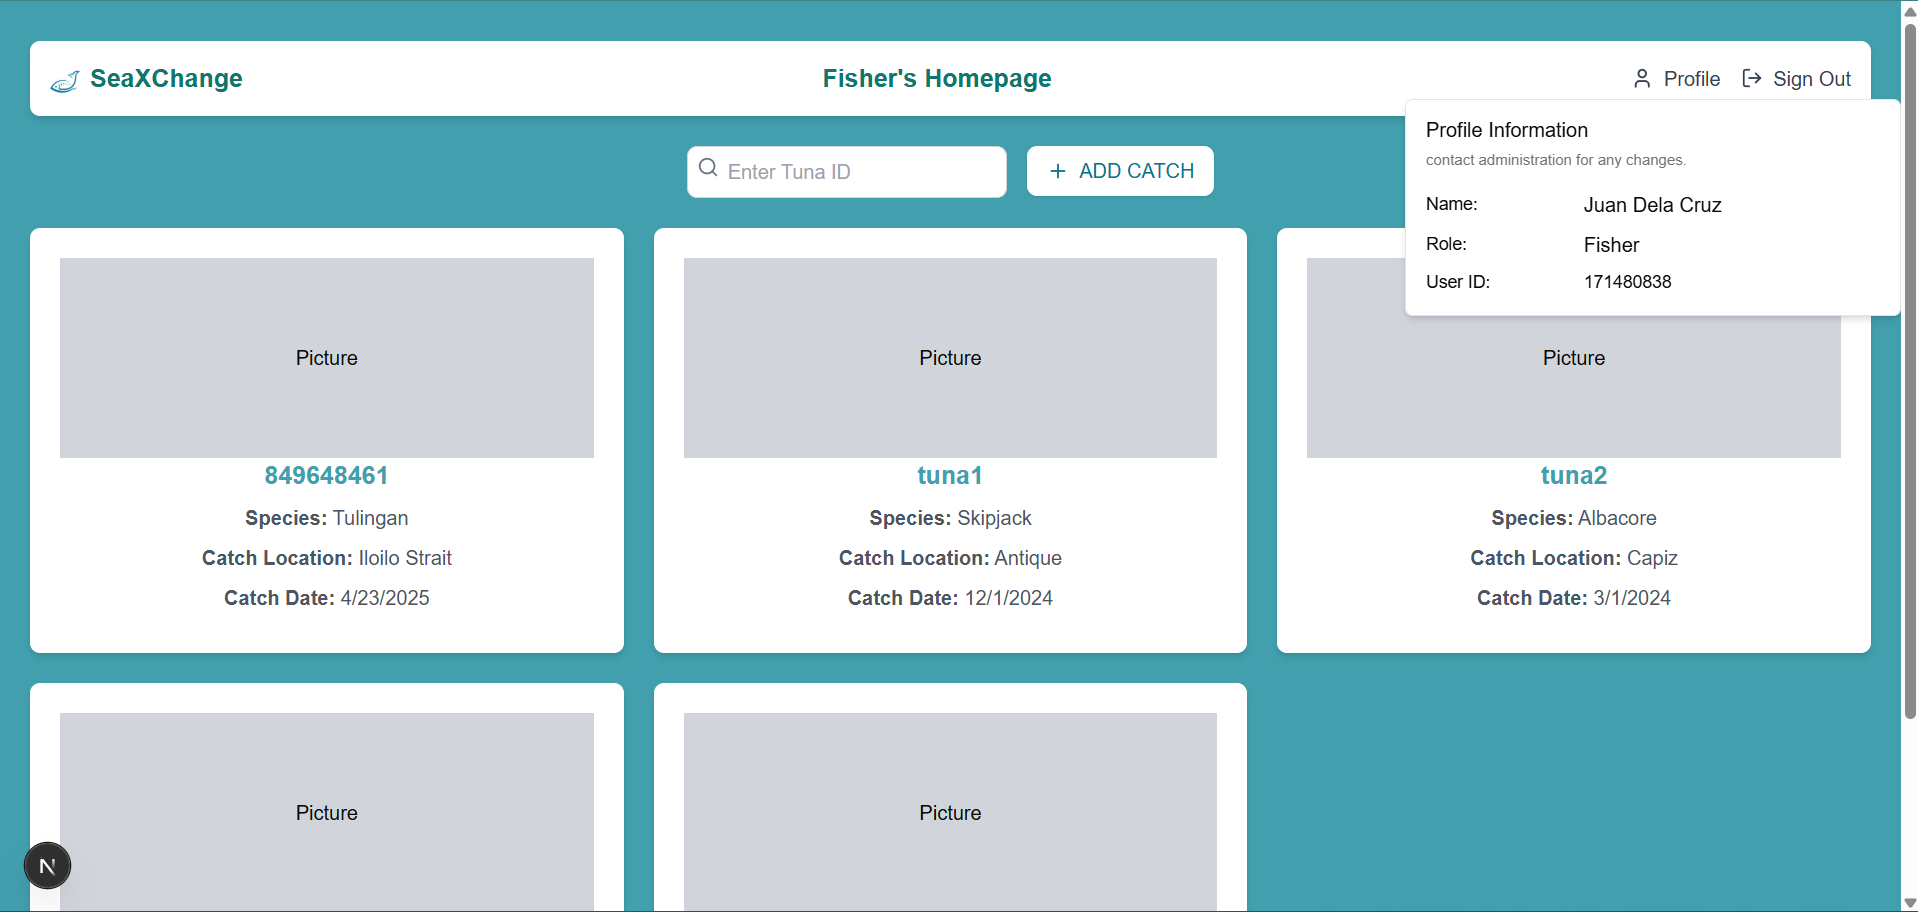
\includegraphics[width=0.8\textwidth]{ProfileHomepage.png}
		\caption{View Profile}
		\label{fig:view_profile}
	\end{figure}

\subsection{Logout}
Users can logout of their accounts and is redirected to the Signup Page.

	\begin{figure}[H]
		\centering
		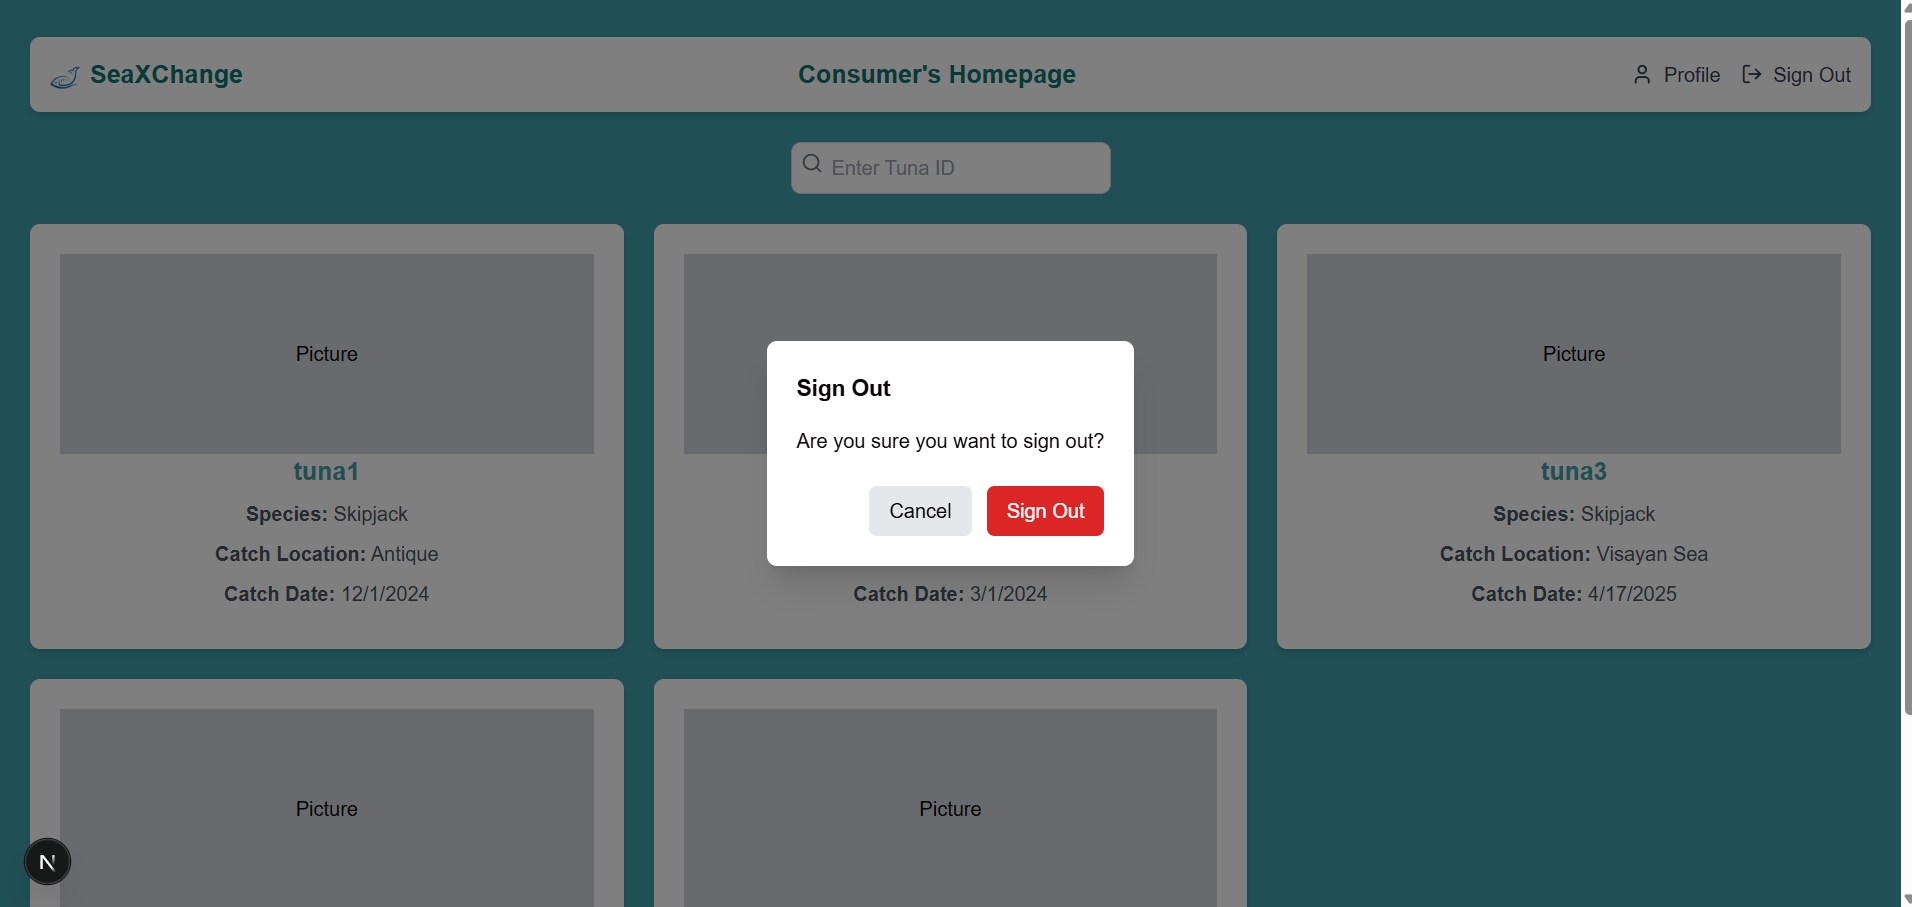
\includegraphics[width=0.8\textwidth]{Signout.png}
		\caption{Log Out}
		\label{fig:signout}
	\end{figure} 
	
\section{System Discussion}
After modifying the Hyperledger Fabric smart contract to assess necessary processes involved in the tuna supply chain, the blockchain is ready to be invoked wherein the smart contract can be activated. To start, a new tuna asset is added and registered to the blockchain. Each tuna asset has its attributes or details. Before proceeding to the transfer of tuna asset, the smart contract is queried to verify if the creation of the asset is successful and if it is part of the current inventory. After that, the tuna asset can be transferred from fisher to supplier and the asset's owner is updated. The smart contract is queried again to verify if the asset details have been updated successfully. With the same process, the tuna asset is transferred from supplier to retailer using the smart contract and the owner is updated again. To ensure that the asset details are successfully updated, the smart contract is queried again. The final step is to query the smart contract to show the overview of all the assets in the supply chain. With this, it can be seen all the tuna assets from fishing to retail. Overall, the steps and process provides transparency and traceability in the tuna supply chain.

\section{User Demonstration and Feedback Results}
\subsection{Demo Setup and Scenario}
	During the demonstration of the system, the participants had a brief introduction of the key functionalities of the SeaXChange app. They were shown how to create an account, input and send tuna assets from one stakeholder to another. Participants were also shown how real-time updates were reflected on the app. Finally, they were introduced on how to view transaction histories and traceability information on each tuna asset. Throughout the demonstration, participants were encouraged to ask questions and provide feedback on the usability and functionality of the system. After the demonstration, they were given feedback forms in order to assess the SeaXChange app. 
	
	\begin{figure}[H]
		\centering
		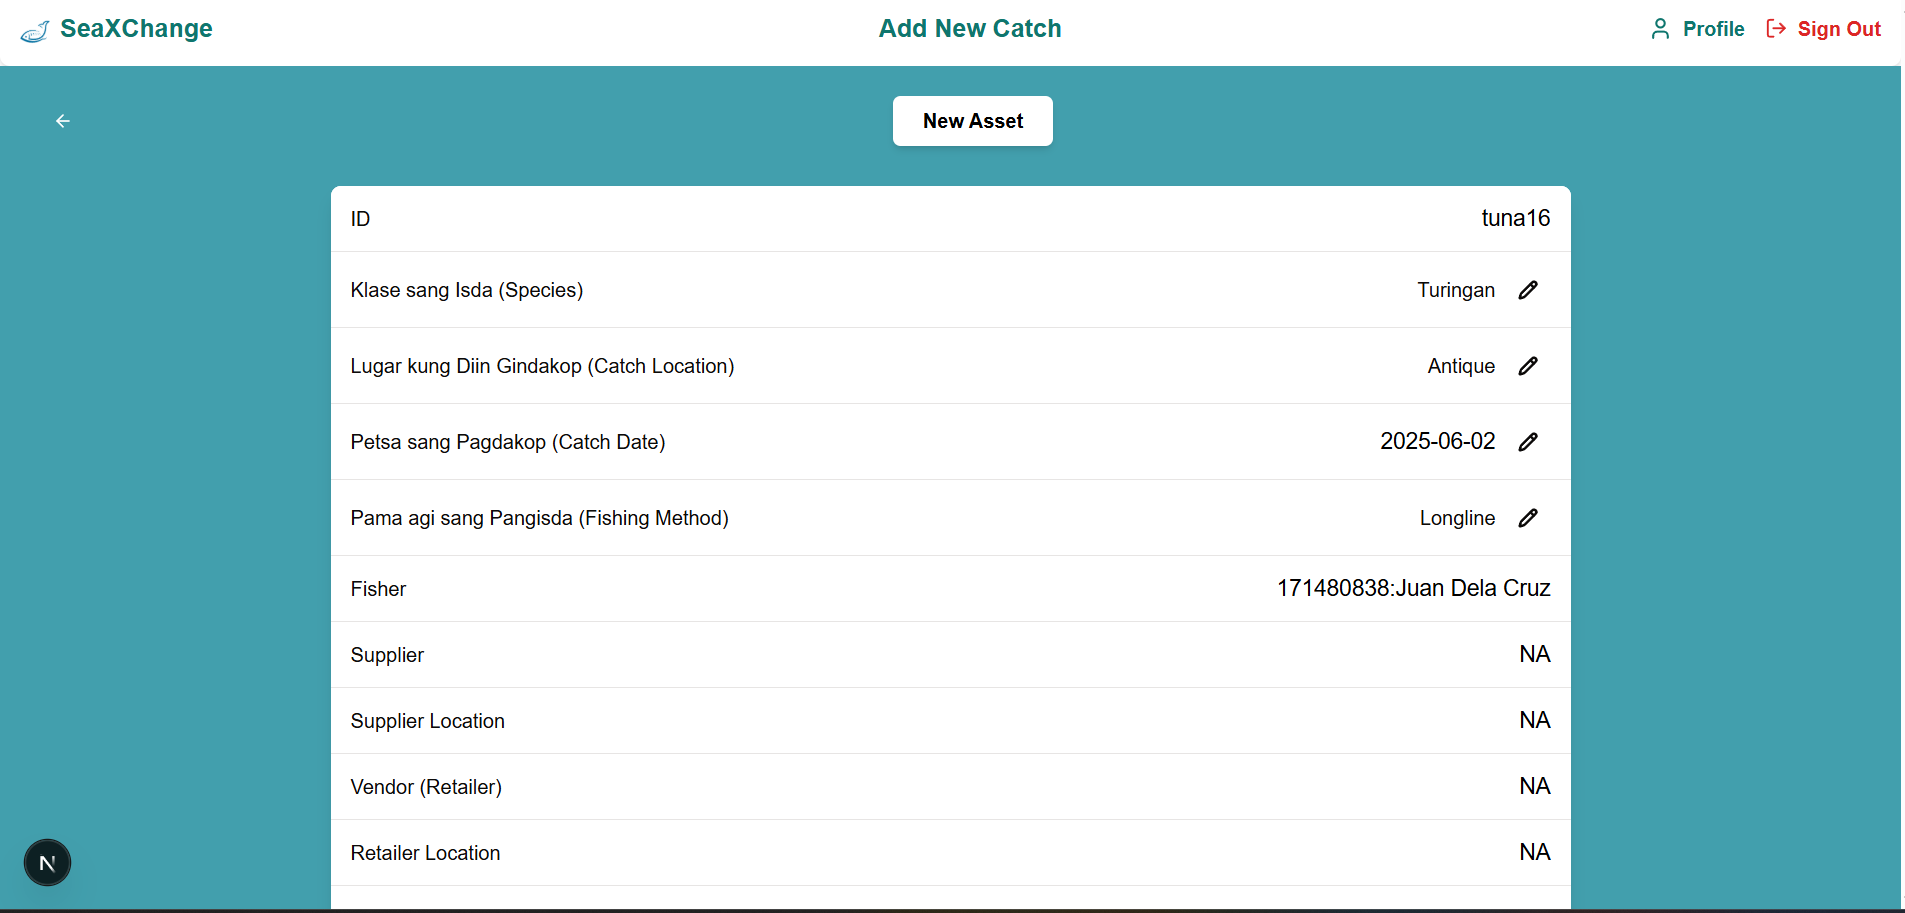
\includegraphics[width=0.8\textwidth]{AddCatch.png}
		\caption{Add Catch (Asset)}
		\label{fig:add_catch}
	\end{figure}
	
	\begin{figure}[H]
		\centering
		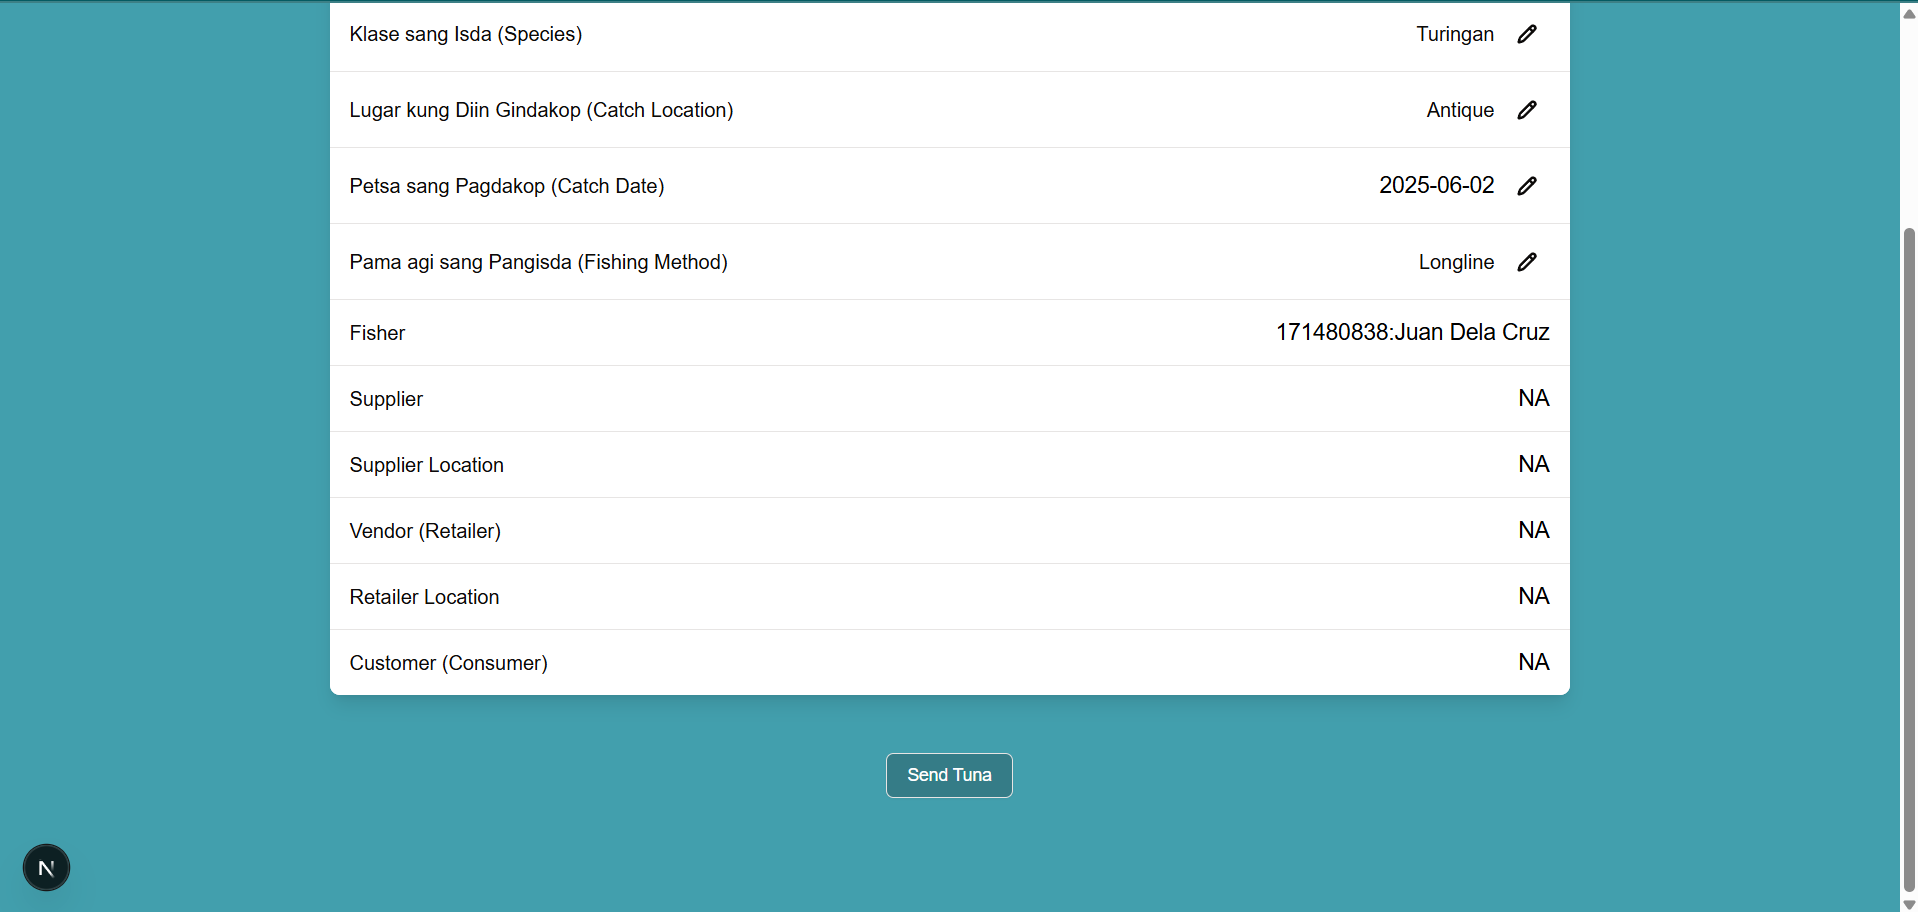
\includegraphics[width=0.8\textwidth]{SaveAddCatch.png}
		\caption{Save Details}
		\label{fig:save_details}
	\end{figure}
	
	\begin{figure}[H]
		\centering
		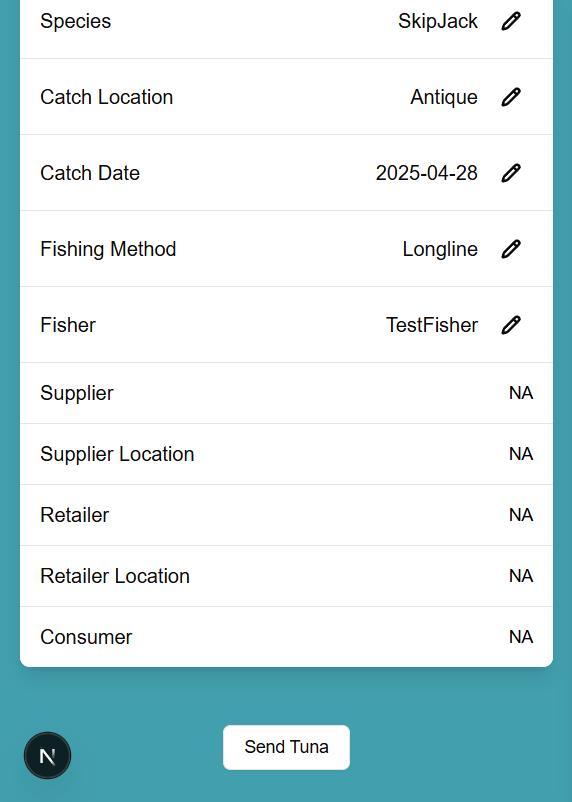
\includegraphics[width=0.8\textwidth]{AfterSaving.png}
		\caption{After Save Details}
		\label{fig:after_save}
	\end{figure}
	
	\begin{figure}[H]
		\centering
		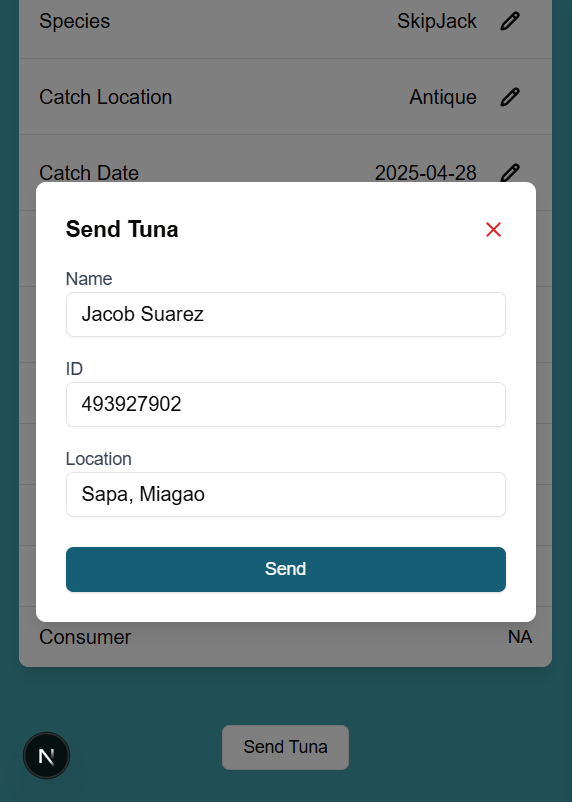
\includegraphics[width=0.8\textwidth]{SendToSupplier.png}
		\caption{Send Asset}
		\label{fig:sendto_supplier}
	\end{figure}
	
\subsection{Feedback Collection Method}
	The feedback was collected through a combination of structured interviews and assessment forms. Participants were asked to complete an assessment rubric evaluating the SeaXChange app across key criteria such as functionality, end-user needs, performance, usability, ease of use and feasibility. Moreover, follow-up interviews were conducted to gather deeper qualitative insights and obtain suggestions for system improvement.
	
	The feedback gathered from fishermen, suppliers and retailers, and consumers was analyzed based on the SeaXChange assessment rubric, which evaluated six major categories: Functionality, End-user Needs, Performance, Usability, Ease of Use and Feasibility. The collected data were analyzed using descriptive statistics, through the computation of mean scores for each assessment criterion. These mean values were used to summarize stakeholder perceptions of the system. Mean ratings were calculated based on the 1-5 Likert Scale where 1 = Poor and 5 = Very Good.
	
\subsection{Summarized Feedback}
	\begin{table}[h]
		\centering
		\begin{tabular}{|l|l|c|l|}
			\hline
			\textbf{Functionality} & \textbf{Stakeholder} & \textbf{Mean} & \textbf{Description} \\ \hline
			\multirow{3}{*}{Track assets} 
			& Entire Group & 3.67 & Average \\ \cline{2-4}
			& Fishermen & 4.0 & Good \\ \cline{2-4}
			& Supplier and Retailers & 3.0 & Average \\ \cline{2-4}
			& Consumers & 4.0 & Good \\ \hline
			
			\multirow{3}{*}{Verify tuna assets} 
			& Entire Group & 3.67 & Average \\ \cline{2-4}
			& Fishermen & 3.33 & Average \\ \cline{2-4}
			& Supplier and Retailers & 4.0 & Good \\ \cline{2-4}
			& Consumers & 3.67 & Average \\ \hline
			
			\multirow{3}{*}{Support real-time updates} 
			& Entire Group & 3.56 & Average \\ \cline{2-4}
			& Fishermen & 3.78 & Average \\ \cline{2-4}
			& Supplier and Retailers & 4.0 & Good \\ \cline{2-4}
			& Consumers & 4.0 & Good \\ \hline
			
			\multirow{3}{*}{Enable smart contract execution} 
			& Entire Group & 3.42 & Average \\ \cline{2-4}
			& Fishermen & 2.33 & Fair \\ \cline{2-4}
			& Supplier and Retailers & 3.25 & Average \\ \cline{2-4}
			& Consumers & 4.67 & Good \\ \hline
			
		\end{tabular}
		\caption{Mean ratings and descriptions for functionality-related features per stakeholder group.}
		\label{tab:functionality}
	\end{table}
	
	When taken as a whole, the respondents have average feedback in asset tracking but when classified by stakeholder, the fishermen (M = 4.0) and consumers (M = 4.0) had good feedback in tracking , while the supplier and retailers have an average rating (M = 3.0). For verifying tuna assets, the entire group has an average feedback. When classified by stakeholder, the fishermen (M = 3.33) and consumers (M = 3.67) have average ratings.  For real-time updates, the respondents, when taken as a whole, have an average feedback. When classified by stakeholder, the fishermen (M = 3.78) have an average rating, while both supplier and retailers (M = 4.0) and consumers (M = 4.0) have good ratings. For smart contract execution, the respondents, when taken as a whole, also have an average feedback. When classified according to stakeholder, the fishermen have a fair rating (M = 2.33), the supplier and retailers have average ratings (M = 3.25) and the consumers have good ratings (M = 4.67).
	
	\begin{table}[h]
		\centering
		\begin{tabular}{|l|l|c|l|}
			\hline
			\textbf{End-user Needs} & \textbf{Stakeholder} & \textbf{Mean} & \textbf{Description} \\ \hline
			\multirow{3}{*}{Provide transparency in tracking} 
			& Entire Group & 3.56 & Average \\ \cline{2-4}
			& Fishermen & 2.67 & Fair \\ \cline{2-4}
			& Supplier and Retailers & 4.0 & Good \\ \cline{2-4}
			& Consumers & 4.0 & Good \\ \hline
			
			\multirow{3}{*}{Provide seamless interaction} 
			& Entire Group & 3.77 & Average \\ \cline{2-4}
			& Fishermen & 1.33 & Poor \\ \cline{2-4}
			& Supplier and Retailers & 3.0 & Average \\ \cline{2-4}
			& Consumers & 4.0 & Good \\ \hline
			
		\end{tabular}
		\caption{Mean ratings and descriptions for end-user needs-related features per stakeholder group.}
		\label{tab:end-user}
	\end{table}
	
	The respondents, when taken as a whole, had an average feedback in transparency. When classified by stakeholder, The fishermen have fair ratings (M = 2.67), while both supplier and retailers (M = 4.0) and consumers (M = 4.0) have good ratings. In evaluating the seamless interaction of the app, the entire group has an average feedback (M = 3.77). When classified by stakeholder, the fishermen (M = 1.33) have poor feedback, the supplier and retailers have average feedback (M = 3.0) and the consumers have good feedback (M = 4.0) in seamless interaction.
	
	\vspace{1cm}
	\begin{table}[h]
		\centering
		\begin{tabular}{|l|l|c|l|}
			\hline
			\textbf{Performance} & \textbf{Stakeholder} & \textbf{Mean} & \textbf{Description} \\ \hline
			\multirow{3}{*}{Processes transactions efficiently} 
			& Entire Group & 3.81 & Average \\ \cline{2-4}
			& Fishermen & 3.67 & Average \\ \cline{2-4}
			& Supplier and Retailers & 3.75 & Average \\ \cline{2-4}
			& Consumers & 4.0 & Good \\ \hline
			
			\multirow{3}{*}{Ensures data integrity and security} 
			& Entire Group & 3.31 & Average \\ \cline{2-4}
			& Fishermen & 2.67 & Fair \\ \cline{2-4}
			& Supplier and Retailers & 3.25 & Average \\ \cline{2-4}
			& Consumers & 4.0 & Good \\ \hline
			
		\end{tabular}
		\caption{Mean ratings and descriptions for performance-related features per stakeholder group.}
		\label{tab:performance}
	\end{table}
	
	As a whole, the respondents have an average feedback on efficient transactions (M = 3.81). If evaluated per stakeholder, both fishermen (M = 3.67), supplier and retailers (M = 3.75) evaluated average while consumers had good feedback (M = 4.0). For data security, the entire group has an average feedback (M = 3.31). The fishermen have fair evaluation (M = 2.67), supplier and retailers (M = 3.25) have an average and consumers have solid scores (M = 4.0).
	
	
	
	\begin{table}[h]
		\centering
		\begin{tabular}{|l|l|c|l|}
			\hline
			\textbf{Usability} & \textbf{Stakeholder} & \textbf{Mean} & \textbf{Description} \\ \hline
			\multirow{3}{*}{Provides intuitive interface} 
			& Entire Group & 3.83 & Average \\ \cline{2-4}
			& Fishermen & 4.0 & Good \\ \cline{2-4}
			& Supplier and Retailers & 3.5 & Average \\ \cline{2-4}
			& Consumers & 4.0 & Good \\ \hline
			
			\multirow{3}{*}{Allows cross-platform accessibility} 
			& Entire Group & 4.14 & Good \\ \cline{2-4}
			& Fishermen & 4.0 & Good \\ \cline{2-4}
			& Supplier and Retailers & 3.75 & Average \\ \cline{2-4}
			& Consumers & 4.67 & Good \\ \hline
			
			\multirow{3}{*}{Clear, structured, and visually appealing info} 
			& Entire Group & 3.80 & Average \\ \cline{2-4}
			& Fishermen & 3.33 & Average \\ \cline{2-4}
			& Supplier and Retailers & 3.75 & Average \\ \cline{2-4}
			& Consumers & 4.33 & Good \\ \hline
			
		\end{tabular}
		\caption{Mean ratings and descriptions for usability-related features per stakeholder group.}
		\label{tab:usability}
	\end{table}
	
	It shows the frequency of intuitive interface among the respondents when taken as a whole is average (M = 3.83). When classified according to stakeholder, both fishermen (M = 4.0) and consumers (M = 4.0) have good ratings, while the supplier and retailers (M = 3.5) have average ratings. For cross-platform usage, the entire group rated good (M = 4.14). When classified according to stakeholder, both fishermen (M = 4.0) and consumers (M = 4.1) also have good ratings, while supplier and retailers (M = 3.75) have average. For visual clarity, the entire group rated average (M = 3.80). When classified by each stakeholder, both fishermen (M = 3.33) and supplier and retailers (M = 3.75) have average ratings, while consumers (M = 4.33)  have good ratings.
	
	\clearpage
	\begin{table}[h]
		\centering
		\begin{tabular}{|l|l|c|l|}
			\hline
			\textbf{Ease of Use} & \textbf{Stakeholder} & \textbf{Mean} & \textbf{Description} \\ \hline
			\multirow{4}{*}{Clear instructions for new users} 
			& Entire Group & 3.89 & Average \\ \cline{2-4}
			& Fishermen & 4.0 & Good \\ \cline{2-4}
			& Supplier and Retailers & 4.0 & Good \\ \cline{2-4}
			& Consumers & 3.67 & Average \\ \hline
			
			\multirow{4}{*}{Uses clear and simple language} 
			& Entire Group & 3.31 & Average \\ \cline{2-4}
			& Fishermen & 4.03 & Good \\ \cline{2-4}
			& Supplier and Retailers & 3.75 & Average \\ \cline{2-4}
			& Consumers & 4.33 & Good \\ \hline
			
		\end{tabular}
		\caption{Mean ratings and descriptions for ease of use-related features per stakeholder group.}
		\label{tab:ease-of-use}
	\end{table}
	
	When taken as a whole, the respondents (M = 3.89) rated instruction clarity as average. When classified by stakeholder, both fishermen (M = 4.0) and supplier and retailers (M = 4.0) have good feedback regarding instruction clarity, while the consumers (M = 3.67) have average feedback. The entire group rated language clarity as average (M = 3.31). When evaluated by each stakeholder, both fishermen (M = 4.03) and consumers (M = 4.33) have good feedback, while supplier and retailers (M = 3.75) have average feedback. 
	
	
	\vspace{1cm}
	\begin{table}[h]
		\centering
		\begin{tabular}{|l|l|c|l|}
			\hline
			\textbf{Feasibility} & \textbf{Stakeholder} & \textbf{Mean} & \textbf{Description} \\ \hline
			\multirow{4}{*}{Integration with tuna industry} 
			& Entire Group & 4.06 & Good \\ \cline{2-4}
			& Fishermen & 4.0 & Good \\ \cline{2-4}
			& Supplier and Retailers & 4.5 & Good \\ \cline{2-4}
			& Consumers & 3.67 & Average \\ \hline
			
			\multirow{4}{*}{Consumer use to track tuna products} 
			& Entire Group & 4.03 & Good \\ \cline{2-4}
			& Fishermen & 4.0 & Good \\ \cline{2-4}
			& Supplier and Retailers & 3.75 & Average \\ \cline{2-4}
			& Consumers & 4.33 & Good \\ \hline
			
		\end{tabular}
		\caption{Mean ratings and descriptions for feasibility-related features per stakeholder group.}
		\label{tab:feasibility}
	\end{table}
	
	When taken as a whole, it shows that the respondents have good feedback in the system integration. When classified by each stakeholder, both the fishermen (M = 4.0) and supplier and retailers (M = 4.5) have good feedback in system integration, while the consumers(M = 3.67) have an average rating. The frequency of consumer use among stakeholders, when taken as a whole, have good feedback (M = 4.03). When analyzed individually, both the fishermen (M = 4.0) and consumers (M = 4.33) have a good rating, while an average rating for the supplier and retailers (M = 3.75).
	 
\subsection{Results and Analysis}	
For functionality, fishermen rated asset tracking positively but identified challenges in real-time updates and smart contract execution. Suppliers and retailers similarly found strengths in verification and real-time updates, although asset tracking averaged slightly lower. Consumers consistently rated functionality highly, particularly appreciating the system's ability to support smart contracts.

\noindent Regarding end-user needs, fishermen provided the lowest ratings, highlighting difficulties with seamless interaction. Suppliers, retailers, and consumers gave higher scores, suggesting that while transparency was generally achieved, the system's ease of interaction required further improvement for all users.

\noindent In terms of performance, fishermen and suppliers reported average transaction efficiency but noted concerns regarding data integrity and security. Consumers, on the other hand, expressed confidence in both areas.

\noindent For  usability, consumers provided the highest ratings, emphasizing the intuitive design and accessibility of the interface. Fishermen and suppliers also rated usability positively but suggested improvements, such as better visual appeal and language localization. Feedbacks suggested incorporating the Karay-a language since most of the potential users uses that language in their everyday lives. Another suggestion was to use capitalization (UI/UX) for the name of the tuna to give more emphasis to it.  

\noindent Ease of use was generally rated positively across all groups. However, feedback highlighted the need for additional user guidance features, including clearer button descriptions and localized instructions for broader accessibility.

\noindent Finally, feasibility was strongly affirmed by all groups. Stakeholders believed the system could be effectively integrated into the existing tuna supply chain and accessed by consumers as a means to monitor tuna products.
	


